\documentclass[12pt]{article}
\usepackage{a4wide}
\usepackage{color, amssymb}
\usepackage[margin=1in]{geometry}
\usepackage[document]{ragged2e}
\usepackage[table]{xcolor}
\usepackage{multirow}
\usepackage[braket, qm]{qcircuit}
\setlength{\arrayrulewidth}{0.5mm}
\setlength{\tabcolsep}{16pt}
\renewcommand{\arraystretch}{1.9}
\usepackage[english,greek]{babel}
\usepackage{braket}
\usepackage{mathtools}
\usepackage{ragged2e}
\renewcommand{\baselinestretch}{1.5}
\input{epsf}
\usepackage{float}
\usepackage{graphicx}
\usepackage{caption}
\usepackage{subcaption}
\usepackage{cancel}
\usepackage{algorithm}
\usepackage[noend]{algpseudocode}

\begin{document}

\greektext

\noindent\rule{\textwidth}{2pt}
\begin{center}
{\bf ΥΠΟΛΟΓΙΣΤΙΚΗ ΓΕΩΜΕΤΡΙΑ}\\ 
{\bf 1o Σετ Ασκήσεων }\\
{\bf Καλαμαράκης Θεόδωρος:} 2018030022\\
\end{center}
\rule{\textwidth}{.5pt}
\noindent

\begin{center}

\end{center}
 
 

\justifying

\section*{Άσκηση 1}
O αλγόριθμος που υλοποιεί την αναζήτηση \textlatin{range query} σε \textlatin{binary search tree} είναι ο παρακάτω  
\textlatin{
\begin{algorithm}[H]
    \caption*{\textlatin{\bf Range query search in binary search tree}}
    \begin{algorithmic}
    \Function{Range query}{$node,low,high,query$}
    \If{$node$ is null}
        \State {\bf return}
    \EndIf
    \If{$low < node.value$ }
        \State RANGE QUERY($node.left,low,high,query$)
    \EndIf
    \If{$low \leq node.value\leq high$ }
        \State $query$.append($node.value$)
    \EndIf
    \If{$node.value<high$ }
    \State RANGE QUERY($node.right,low,high,query$)
\EndIf
    \EndFunction
    \end{algorithmic}
    \end{algorithm}
}
Ο αλγόριθμος αρχικά, εκτελεί αναζήτηση στο δέντρο προκειμένου να βρεί το κάτω όριo του \textlatin{range query} (δηλαδή το πρώτο  του στοιχείο). Η αναζήτηση σε δυαδικό δέντρο γίνεται σε χρόνο $O(h)$.
Αφού βρεί το κάτω όριο μέτα συνεχίζει ανακτώντας ένα ένα τα υπόλοιπα στοιχεία του \textlatin{query} απο το μικρότερο στο μεγαλύτερο. Ξεκινώντας απο το κάτω όριο, η ανάκτηση του κάθε στοιχείου χρειάζεται $O(1)$ χρόνο
εφόσον θα βρίσκεται ήδη στο αμέσως προηγούμενο στοιχείο, και κάθε στοιχείο προσπελαύνεται ακριβώς μια φορα. Άρα η διαδικασία αυτή χρειάζεται χρόνο $kO(1) = O(k)$ για να ολοκληρωθεί. 
Συνεπώς ο συνολικός χρόνος του αλγορίθμου είναι $O(h+k)$\\
\rule{\textwidth}{.5pt}
\section*{Άσκηση 2}
Χρειάζεται να αποδείξουμε τον ευθή και τον αντίστροφο ισχυρισμό.
\begin{enumerate}
\item Αν τα τμήματα $\overline{p_1p_2}$ και $\overline{q_1q_2}$ τέμνονται, τότε το πολύγονο $[p_1,q_1,p_2,q_2]$ είναι κυρτό.
\item Αν το πολύγονο $[p_1,q_1,p_2,q_2]$ είναι κυρτό, τότε τα $\overline{p_1p_2}$ και $\overline{q_1q_2}$ τέμνονται 
\end{enumerate}
Για τον εύθή ισχυρισμό:
Έστω οτι τα τμήματα $\overline{p_1p_2}$ και $\overline{q_1q_2}$ τέμνονται στο σημείο $X$.
\begin{figure}[H]

    \centering
    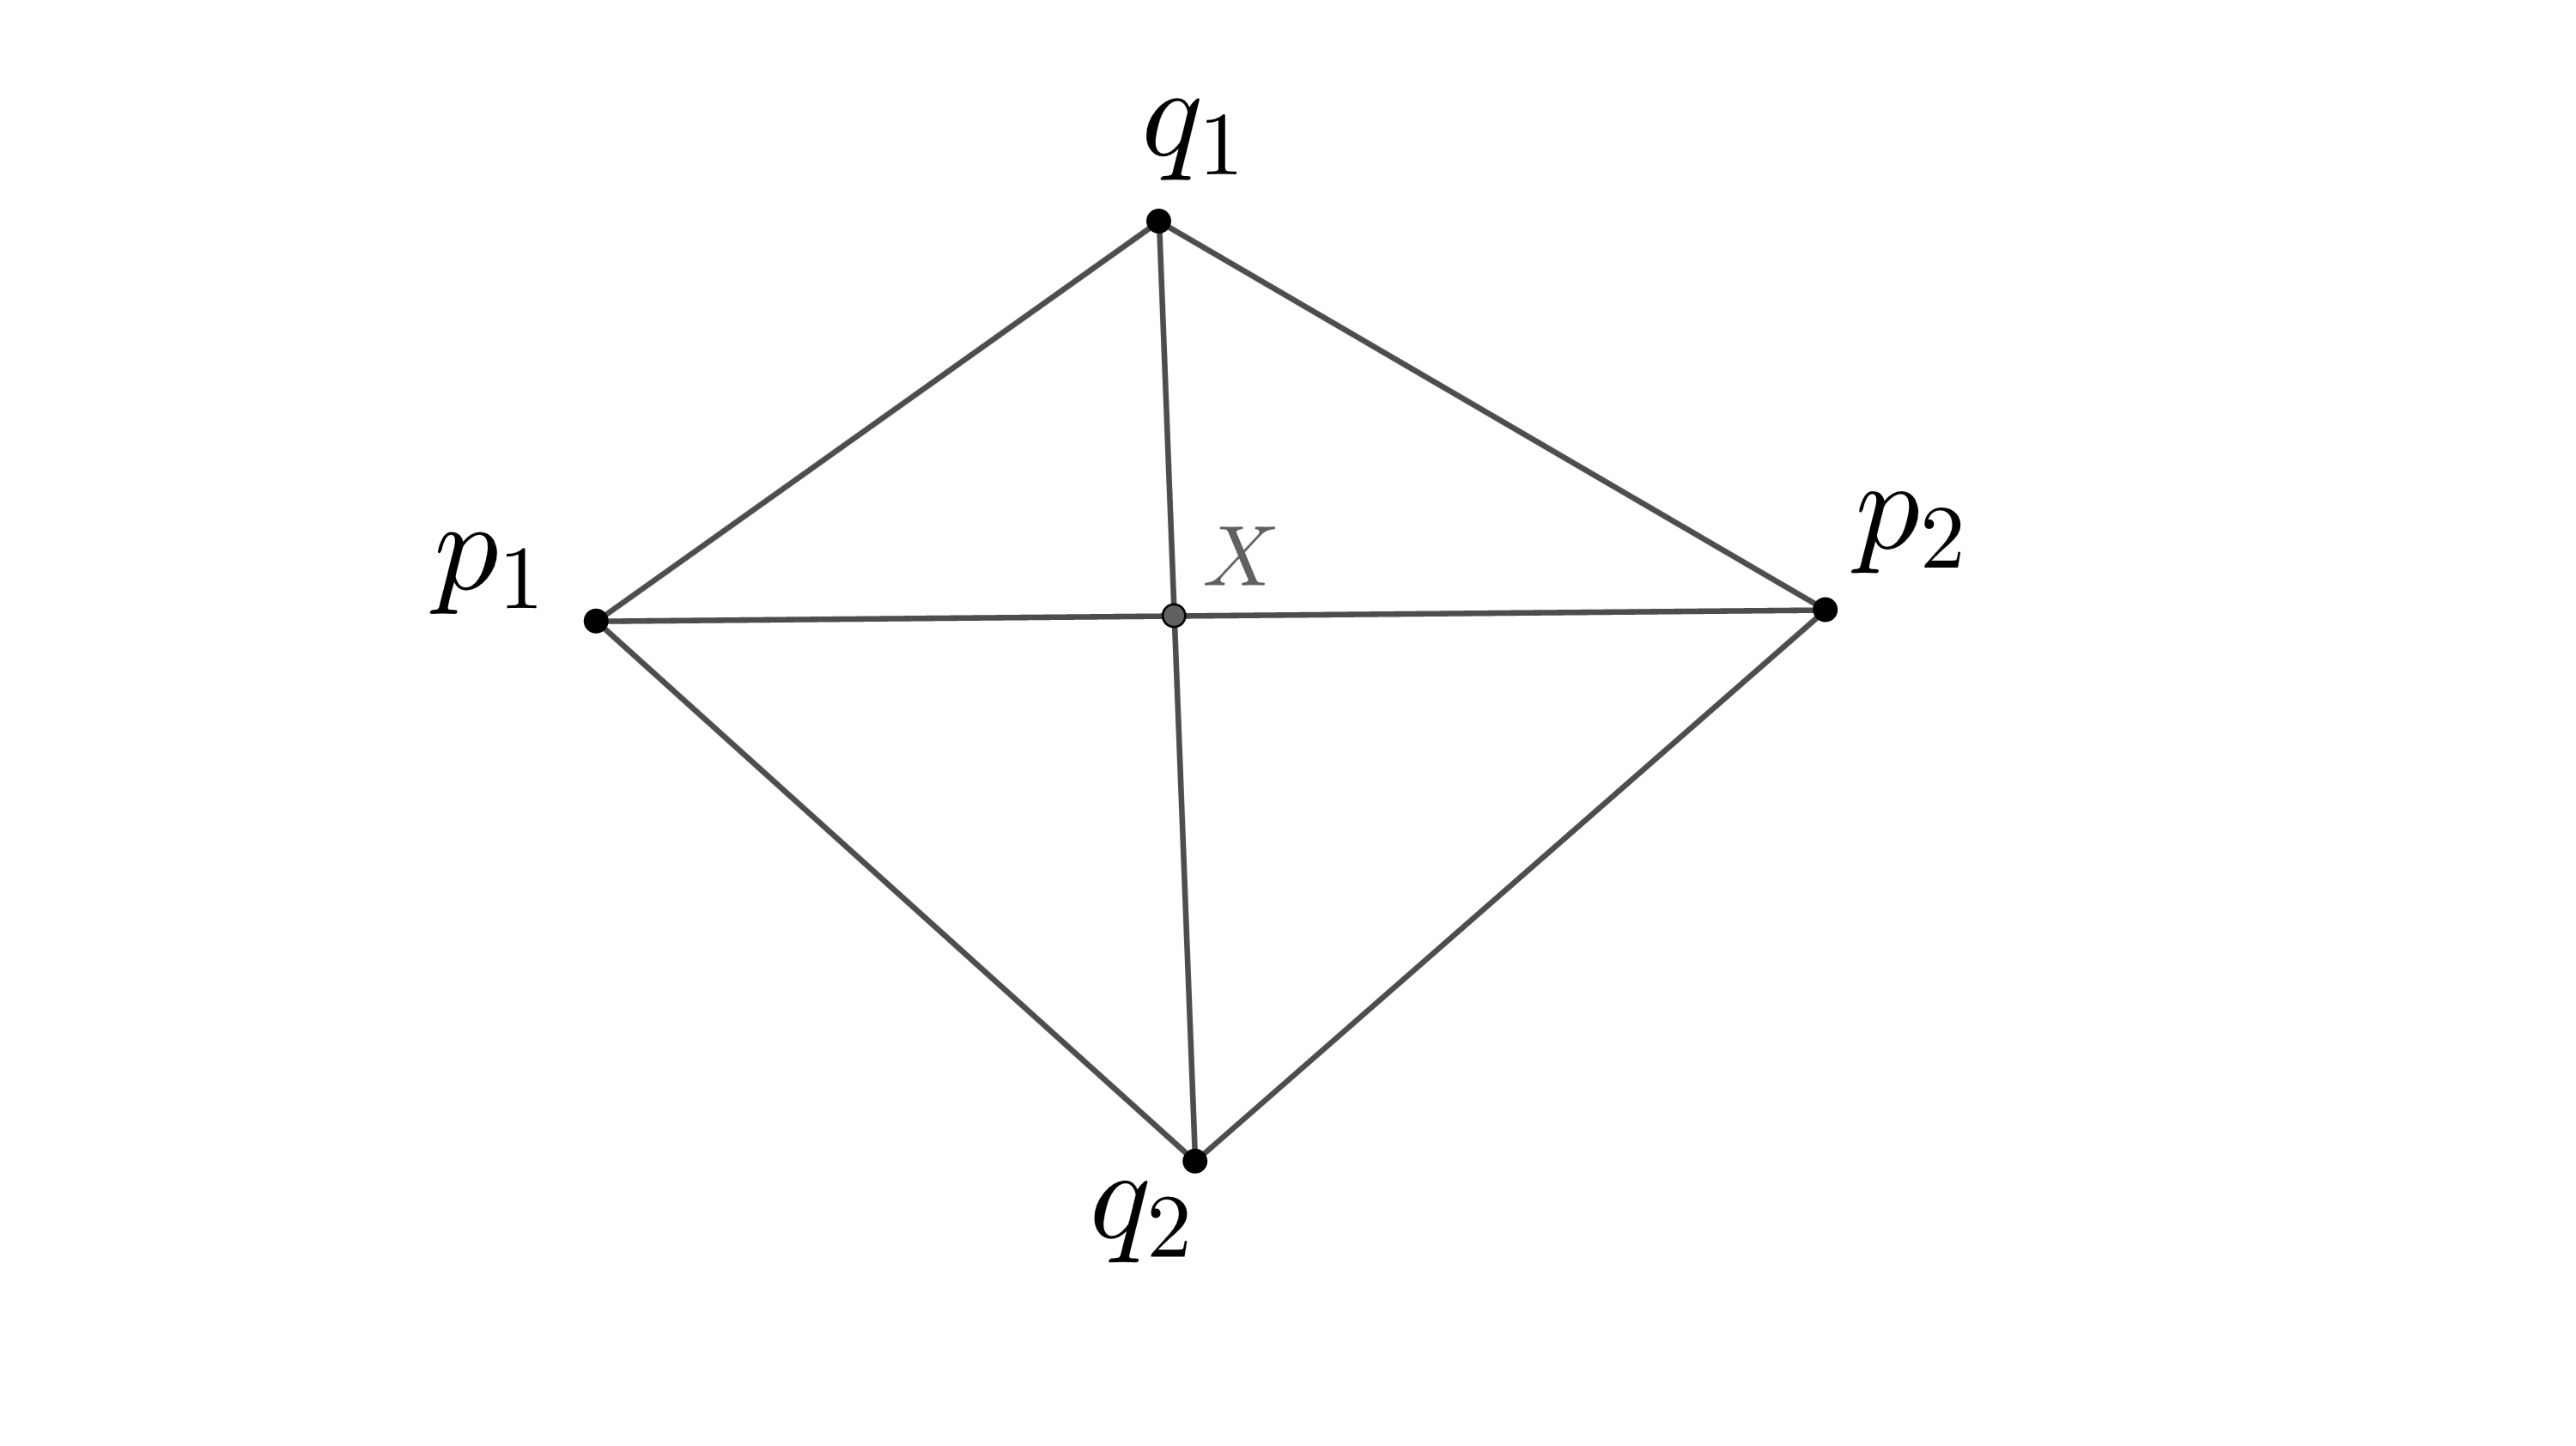
\includegraphics[scale = 1]{geogebra-export.png}\\ 
\end{figure}
Για να αποδείξουμε οτι το $[p_1,q_1,p_2,q_2]$ είναι κυρτό, αρκεί να δείξουμε οτι για κάθε πλεύρα, τα υπολοίπα σημεία του πολυγόνου βρίσκονται δεξιά της.
Π.χ για την πλευρά $\overrightarrow{p_1q_1}$ θέλουμε να δείξουμε οτι $\overrightarrow{p_1q_1}\times \overrightarrow{q_1p_2}<0$ και $\overrightarrow{p_1q_1}\times \overrightarrow{q_1q_2}<0$\\
\begin{itemize}
    \item Αρχικά για να δείξουμε οτι $\overrightarrow{p_1q_1}\times \overrightarrow{q_1p_2}<0$ μπορούμε να γράψουμε οτι $\overrightarrow{p_1q_1} =\overrightarrow{p_1X} + \overrightarrow{Xq_1}  $ και $\overrightarrow{q_1p_2} =\overrightarrow{q_1X} + \overrightarrow{Xp_2}$\\
    Άρα 
    \begin{align*}
            \overrightarrow{p_1q_1}\times \overrightarrow{q_1p_2} &= (\overrightarrow{p_1X} + \overrightarrow{Xq_1}) \times (\overrightarrow{q_1X} + \overrightarrow{Xp_2}) = \\
            &=\overrightarrow{p_1X}\times \overrightarrow{q_1X} + \cancelto{0}{\overrightarrow{p_1X}\times \overrightarrow{Xp_2}} + \cancelto{0}{\overrightarrow{Xq_1}\times \overrightarrow{q_1X}} + \overrightarrow{Xq_1}\times \overrightarrow{Xp_2} = \\
            &=\overrightarrow{p_1X}\times \overrightarrow{q_1X} + \overrightarrow{Xq_1}\times \overrightarrow{Xp_2} < 0
    \end{align*}
    Η τελευταία ανισότητα ισχύει διότι, όπως φαίνεται στο παρακάτω σχήμα $\overrightarrow{p_1X}\times \overrightarrow{q_1X}<0$ και $\overrightarrow{Xq_1}\times \overrightarrow{Xp_2} < 0$, λόγω των δεξιόστροφων γωνιών.
    \begin{figure}[H]

        \centering
        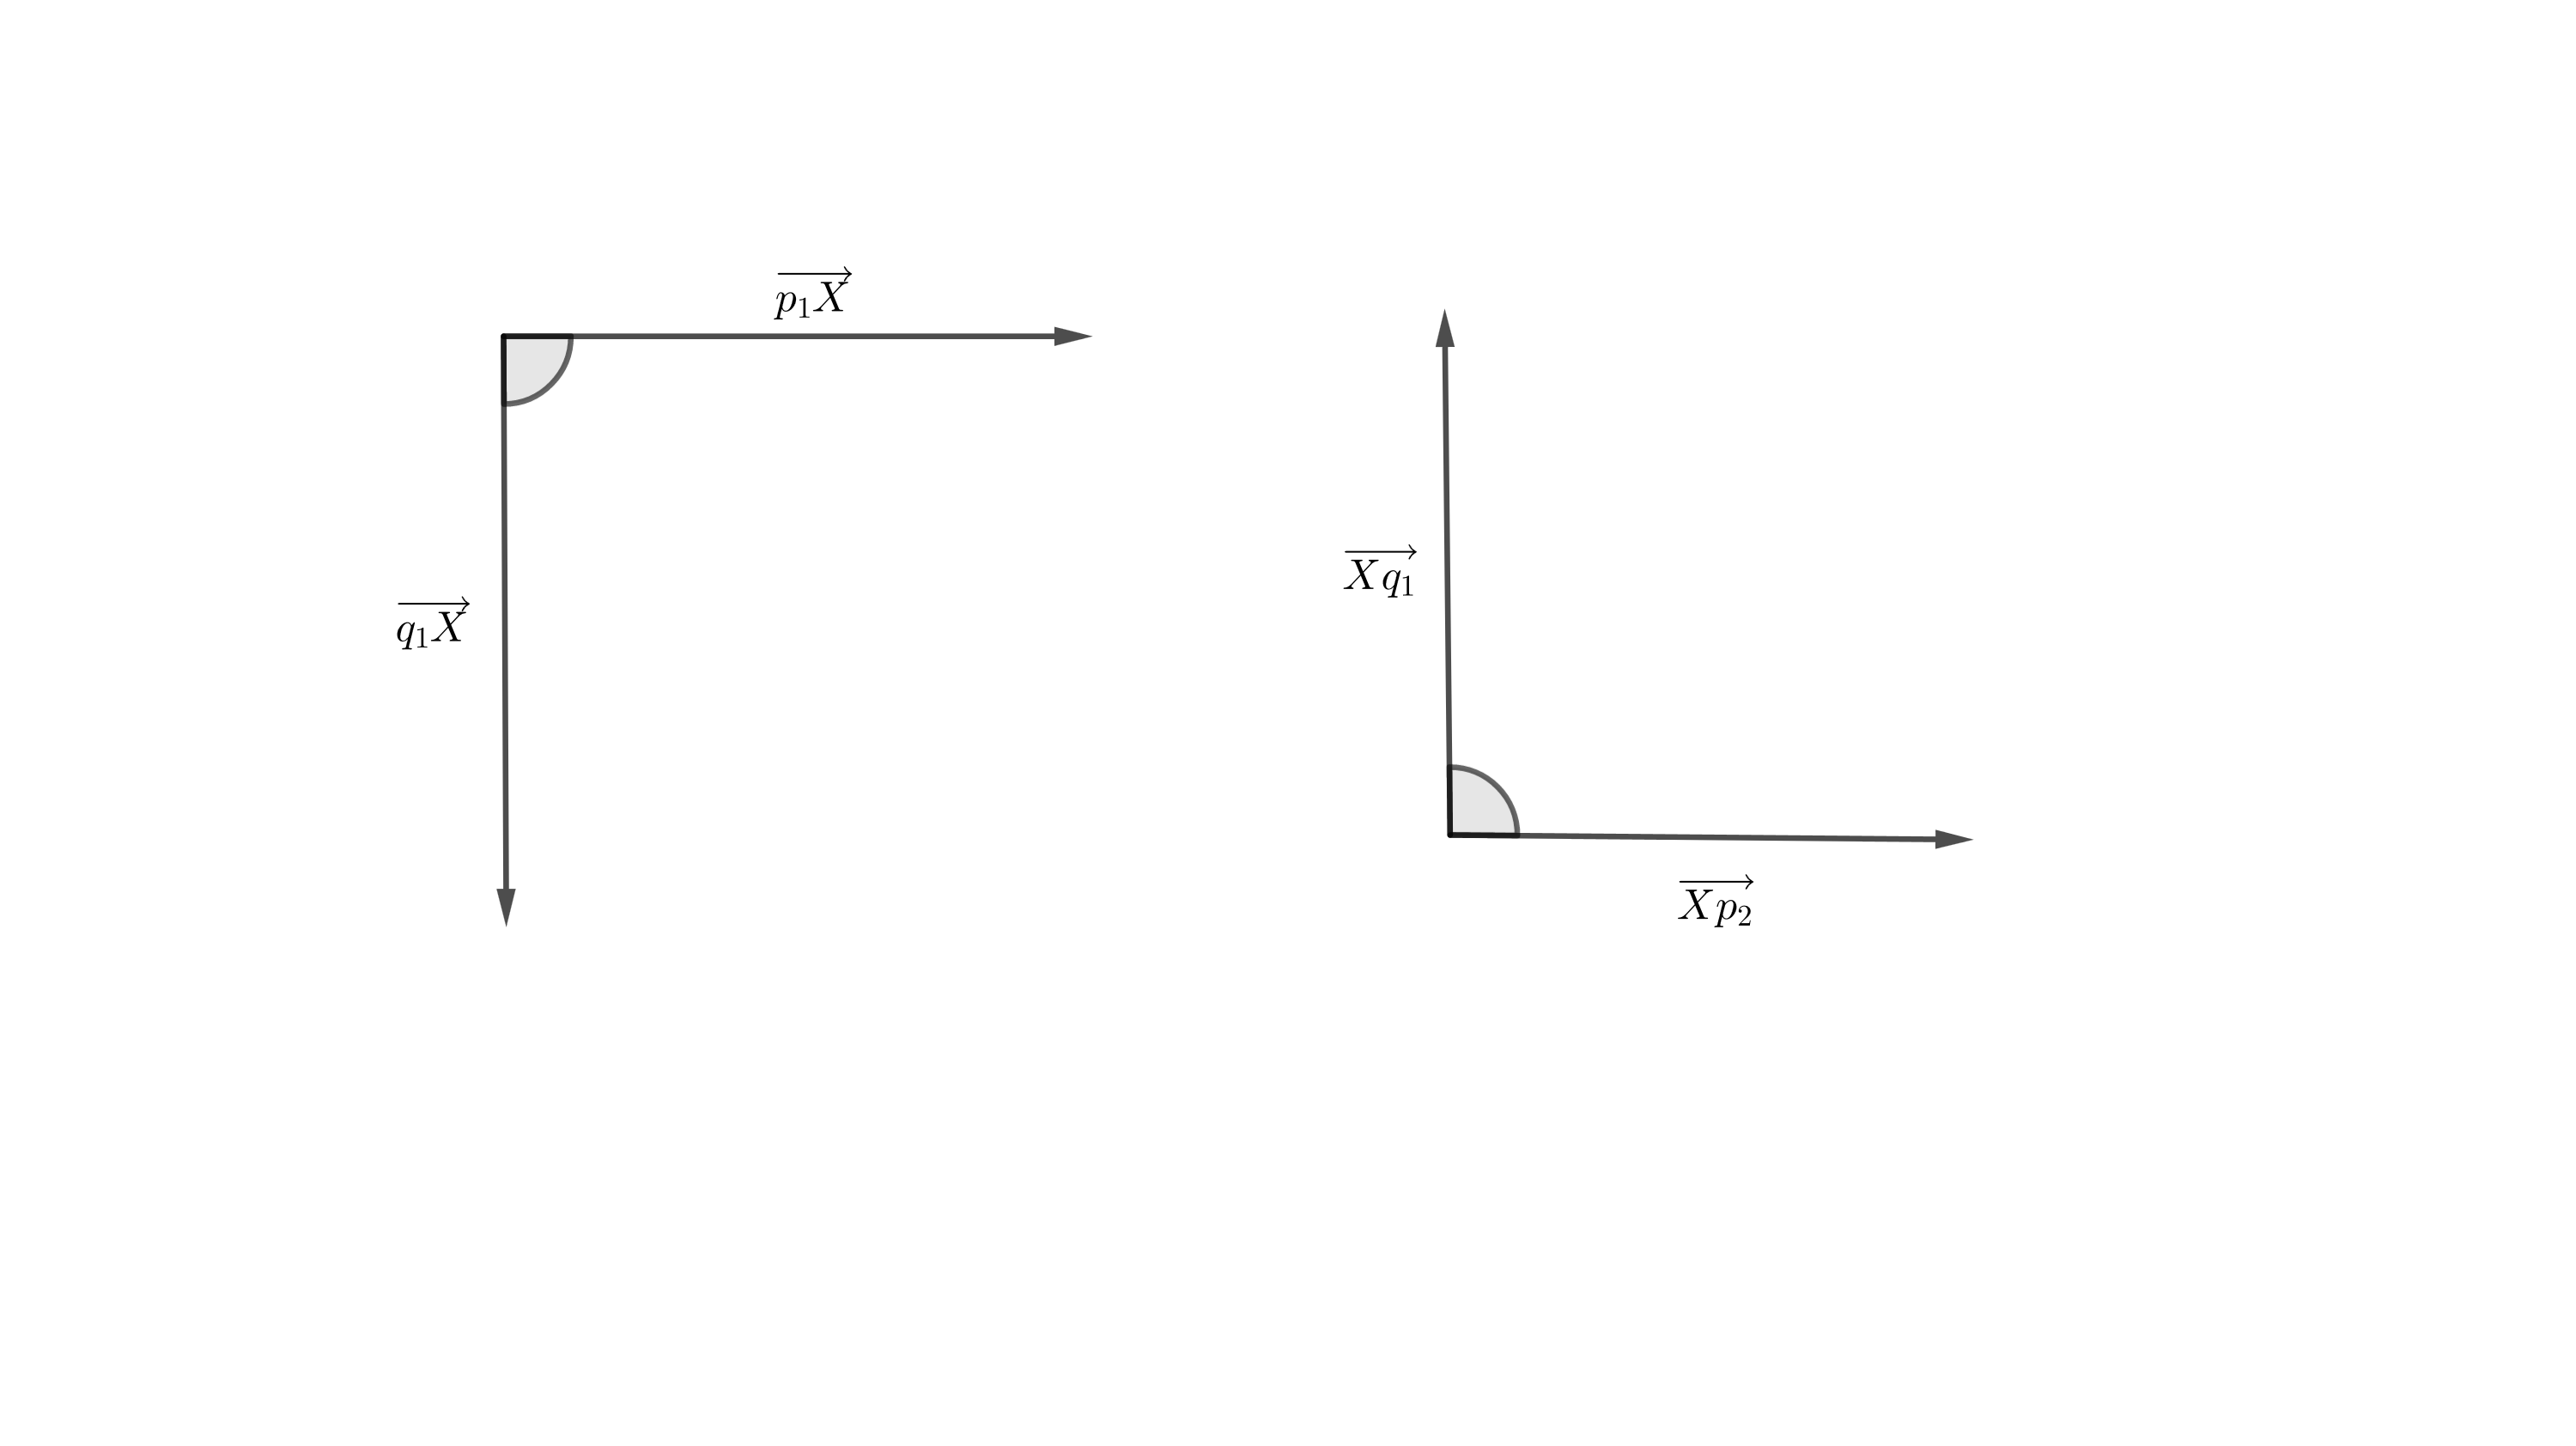
\includegraphics[scale = 1]{ge1.png}\\ 
    \end{figure}
    \item Ομοίως, για να δείξουμε οτι $\overrightarrow{p_1q_1}\times \overrightarrow{q_1q_2}<0$, γράφουμε $\overrightarrow{p_1q_1} =\overrightarrow{p_1X} + \overrightarrow{Xq_1}  $ και $\overrightarrow{q_1q_2} =\overrightarrow{q_1X} + \overrightarrow{Xq_2}$\\
    Άρα 
    \begin{align*}
            \overrightarrow{p_1q_1}\times \overrightarrow{q_1q_2} &= (\overrightarrow{p_1X} + \overrightarrow{Xq_1}) \times (\overrightarrow{q_1X} + \overrightarrow{Xq_2}) = \\
            &=\overrightarrow{p_1X}\times \overrightarrow{q_1X} + \overrightarrow{p_1X}\times \overrightarrow{Xq_2} + \cancelto{0}{\overrightarrow{Xq_1}\times \overrightarrow{q_1X}} + \cancelto{0}{\overrightarrow{Xq_1}\times \overrightarrow{Xq_2}} = \\
            &=\overrightarrow{p_1X}\times \overrightarrow{q_1X} + \overrightarrow{p_1X}\times \overrightarrow{Xq_2} < 0
    \end{align*}
    Oπως και πριν, η τελευταία ανισότητα ισχύει διότι, $\overrightarrow{p_1X}\times \overrightarrow{q_1X}<0$ και $\overrightarrow{p_1X}\times \overrightarrow{Xq_2} < 0$, λόγω των δεξιόστροφων γωνιών.

\end{itemize}
Συνεπώς αποδείξαμε οτι τα σημεία $p_2$ και $q_2$ βρίσκονται στον δεξή ημιχώρο που ορίζεται απο την πλεύρα $\overline{p_1q_1}$. Eφαρμόζοντας την ίδια διαδικασία για τις άλλες τρείς πλευρές, αποδεικνύεται οτι το πολύγονο $[p_1,q_1,p_2,q_2]$ είναι κυρτό.\\

Για τον αντίστροφο ισχυρισμό: Έστω οτι το πολύγονο $[p_1,q_1,p_2,q_2]$ είναι κυρτό.
Tότε το σημείο $q_2$ θα βρίσκεται δέξια το τμήματος $\overrightarrow{q_1p_2}$  και δεξιά του τμήματος $\overrightarrow{p_1q_1}$, δηλαδή θα βρίσκεται στην υποχώρο $S$ όπως φαίνεται στο παρακάτω σχήμα.
\begin{figure}[H]

    \centering
    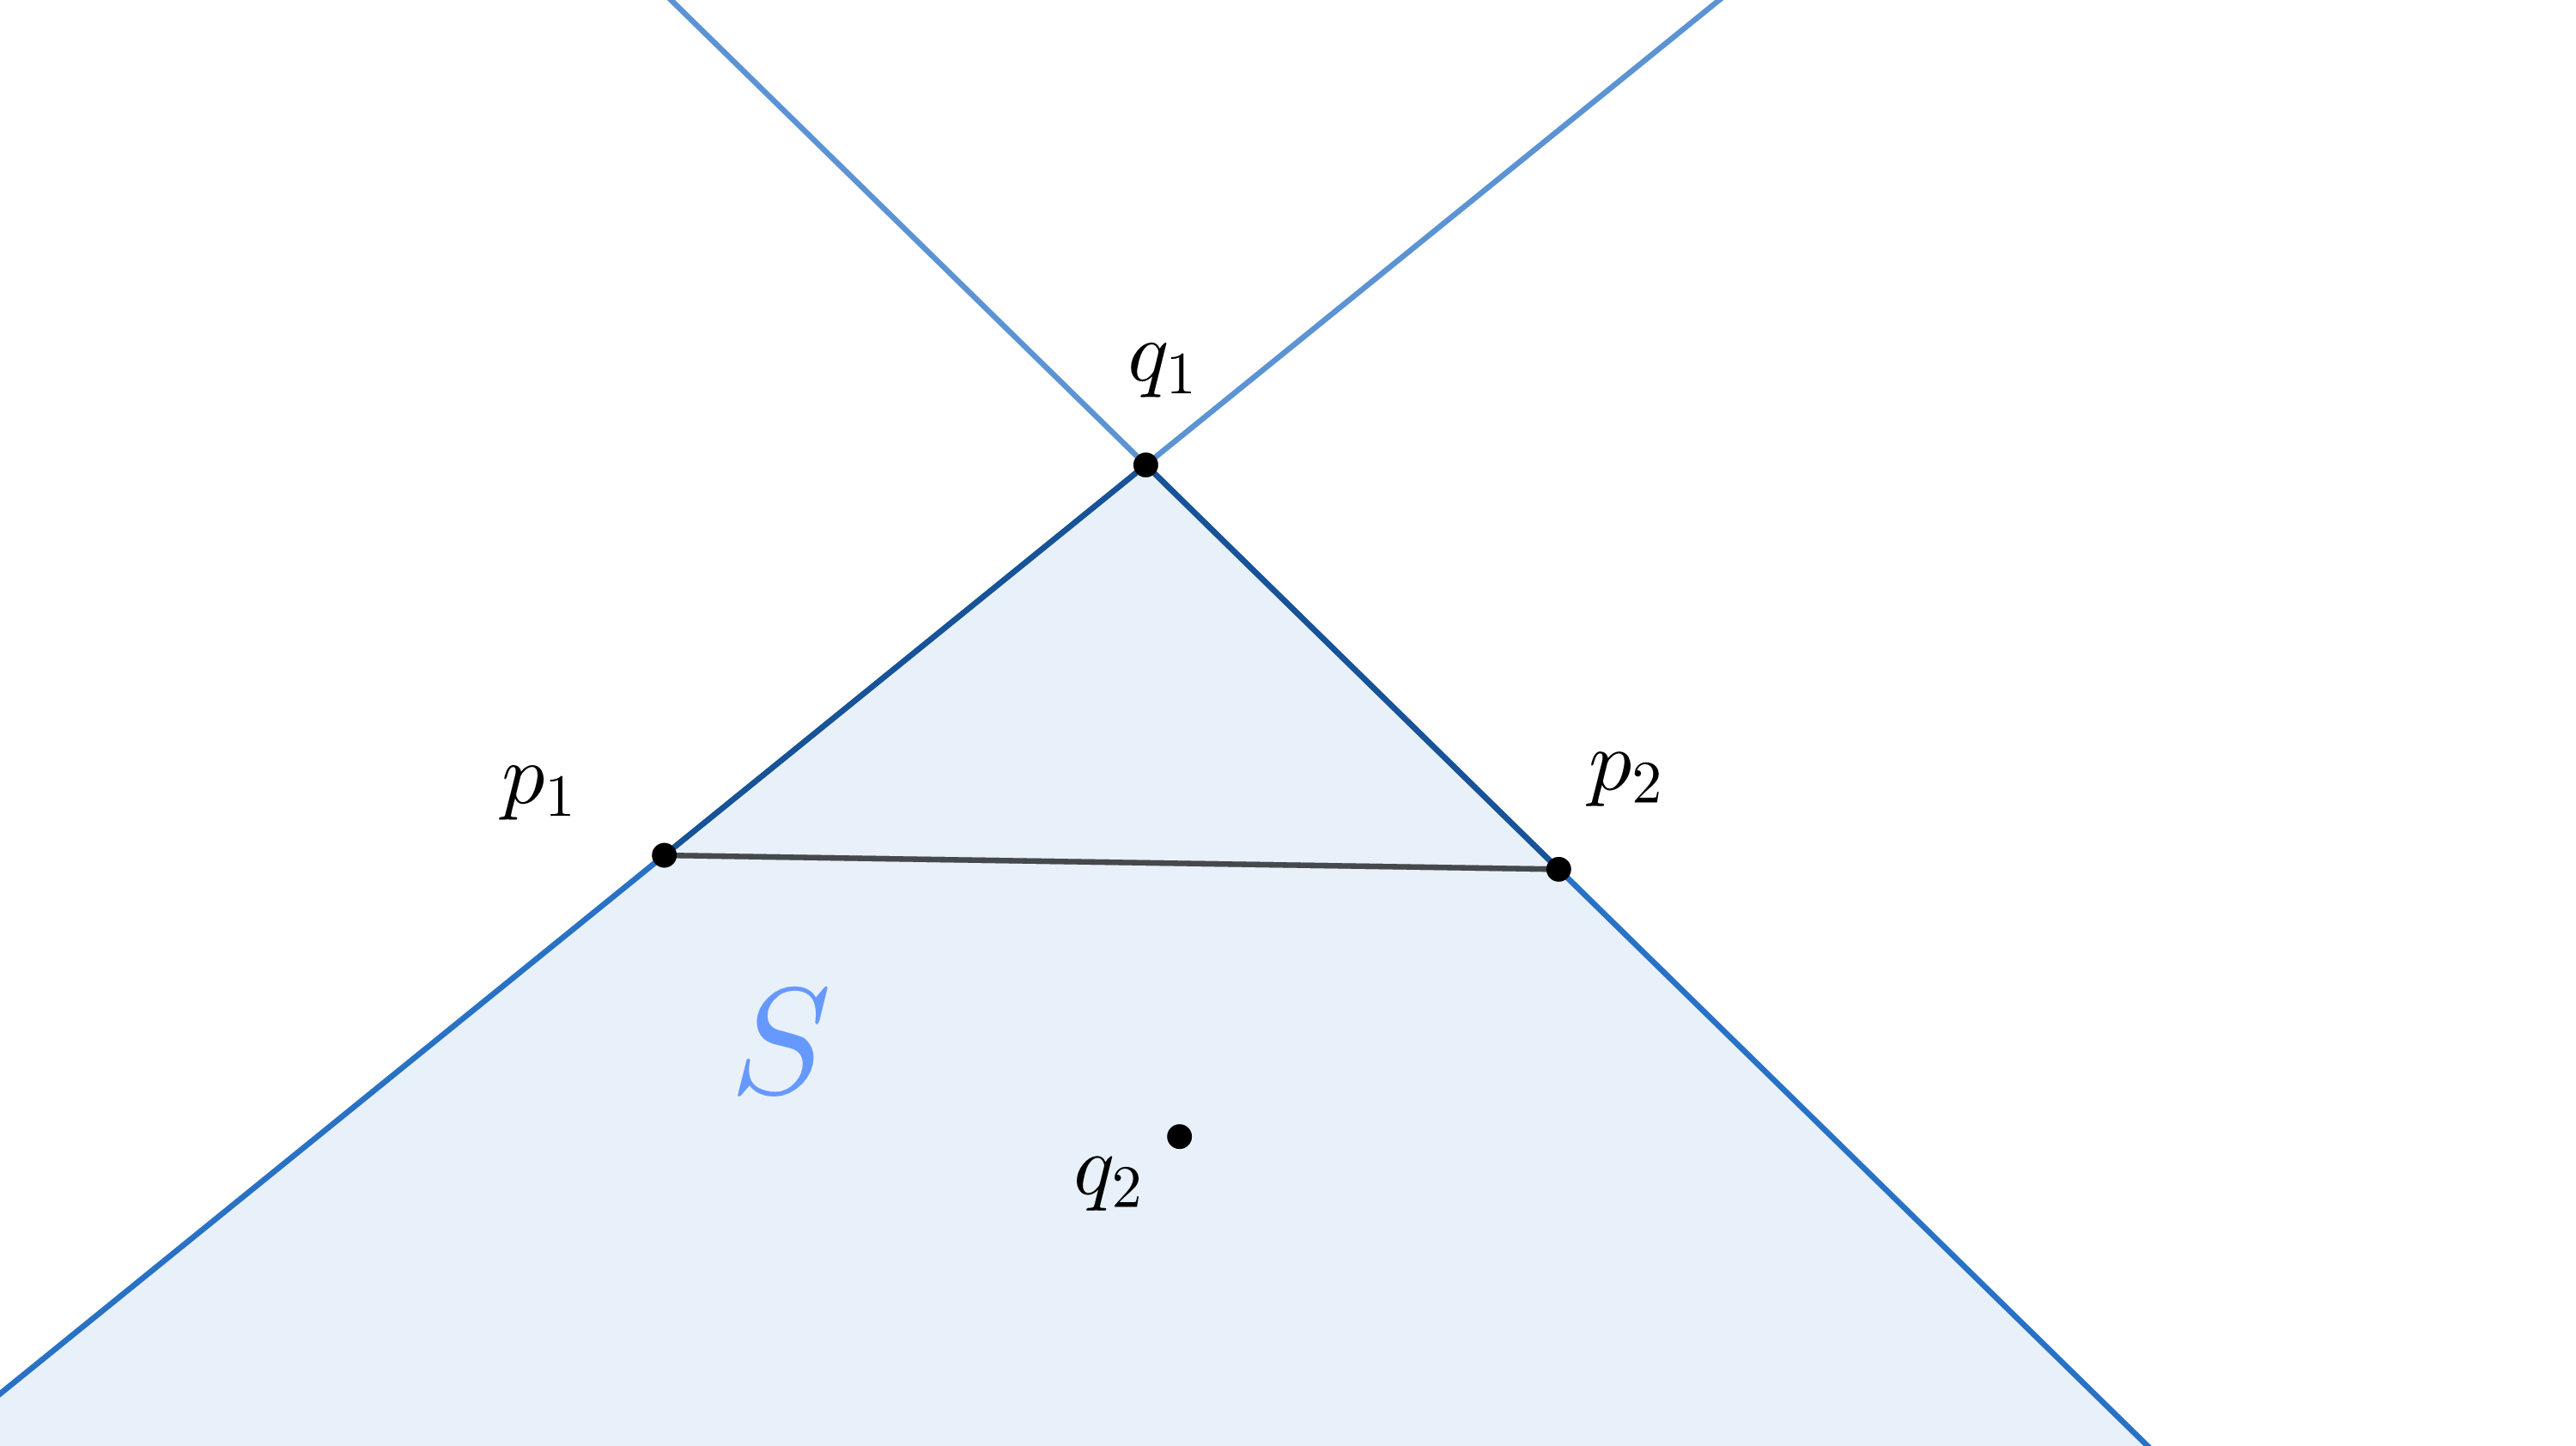
\includegraphics[scale = 0.6]{ge2.png}\\ 
\end{figure}
 Εάν το $q_2$  βρίσκεται πάνω απο το τμήμα  $\overline{p_1p_2}$  μέσα στον υποχώρο $S_1$ που ορίζεται απο το τρίγωνο $p_1q_1p_2$, τότε το τμήμα  $\overline{p_1p_2}$ θα βρίσκεται εκτός του πολυγόνου  $[p_1,q_1,p_2,q_2]$, το όποίο είναι άτοπο κάθως έχουμε υποθέσει οτι το πολύγονο είναι κυρτό (εφόσον $p_1,p_2$ ανήκουν στο πολύγονο θα πρέπει και το τμήμα $\overline{p_1p_2}$ να ανήκει  )
 \begin{figure}[H]

    \centering
    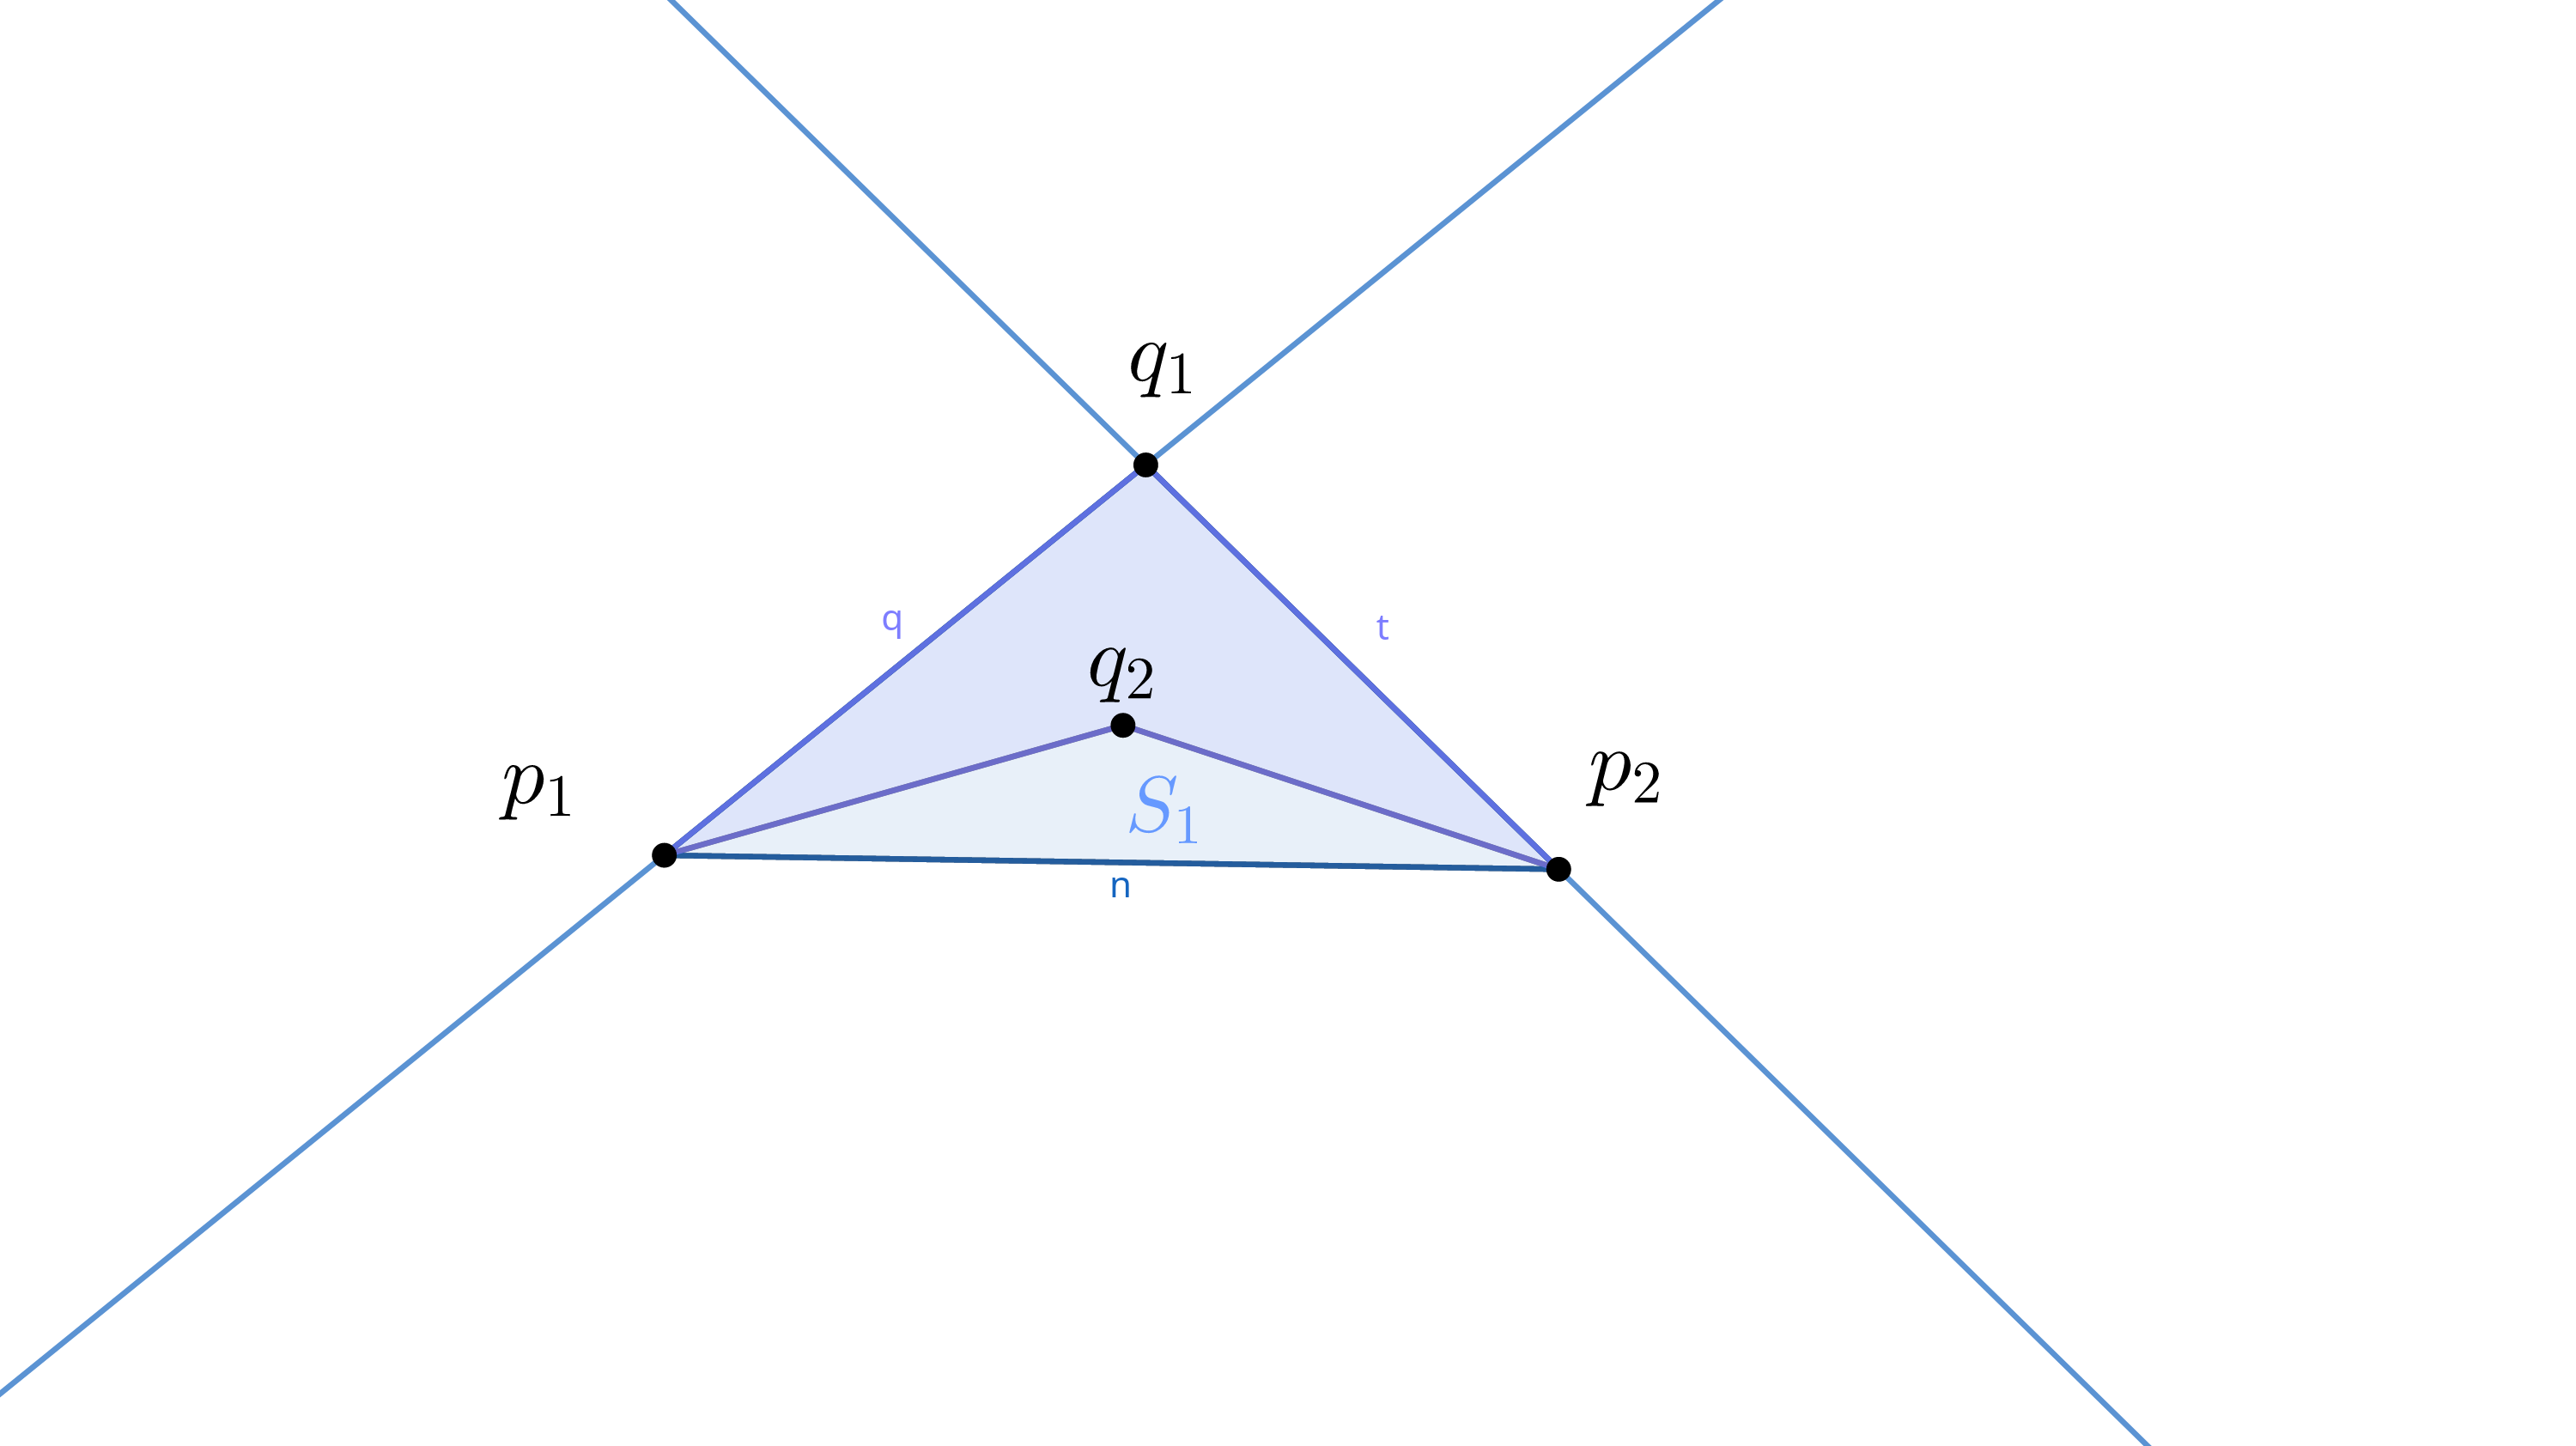
\includegraphics[scale = 0.6]{ge3.png}\\ 
\end{figure} 
Άρα το $q_2$ βρίσκεται σίγουρα στον υποχώρο $S_2$ και κατα συνέπεια το τμήμα $\overline{q_1q_2}$  τέμνει σίγουρα το τμήμα $\overline{p_1p_2}$, όπως φαίνεταιστο παρακάτω σχήμα.
\begin{figure}[H]

    \centering
    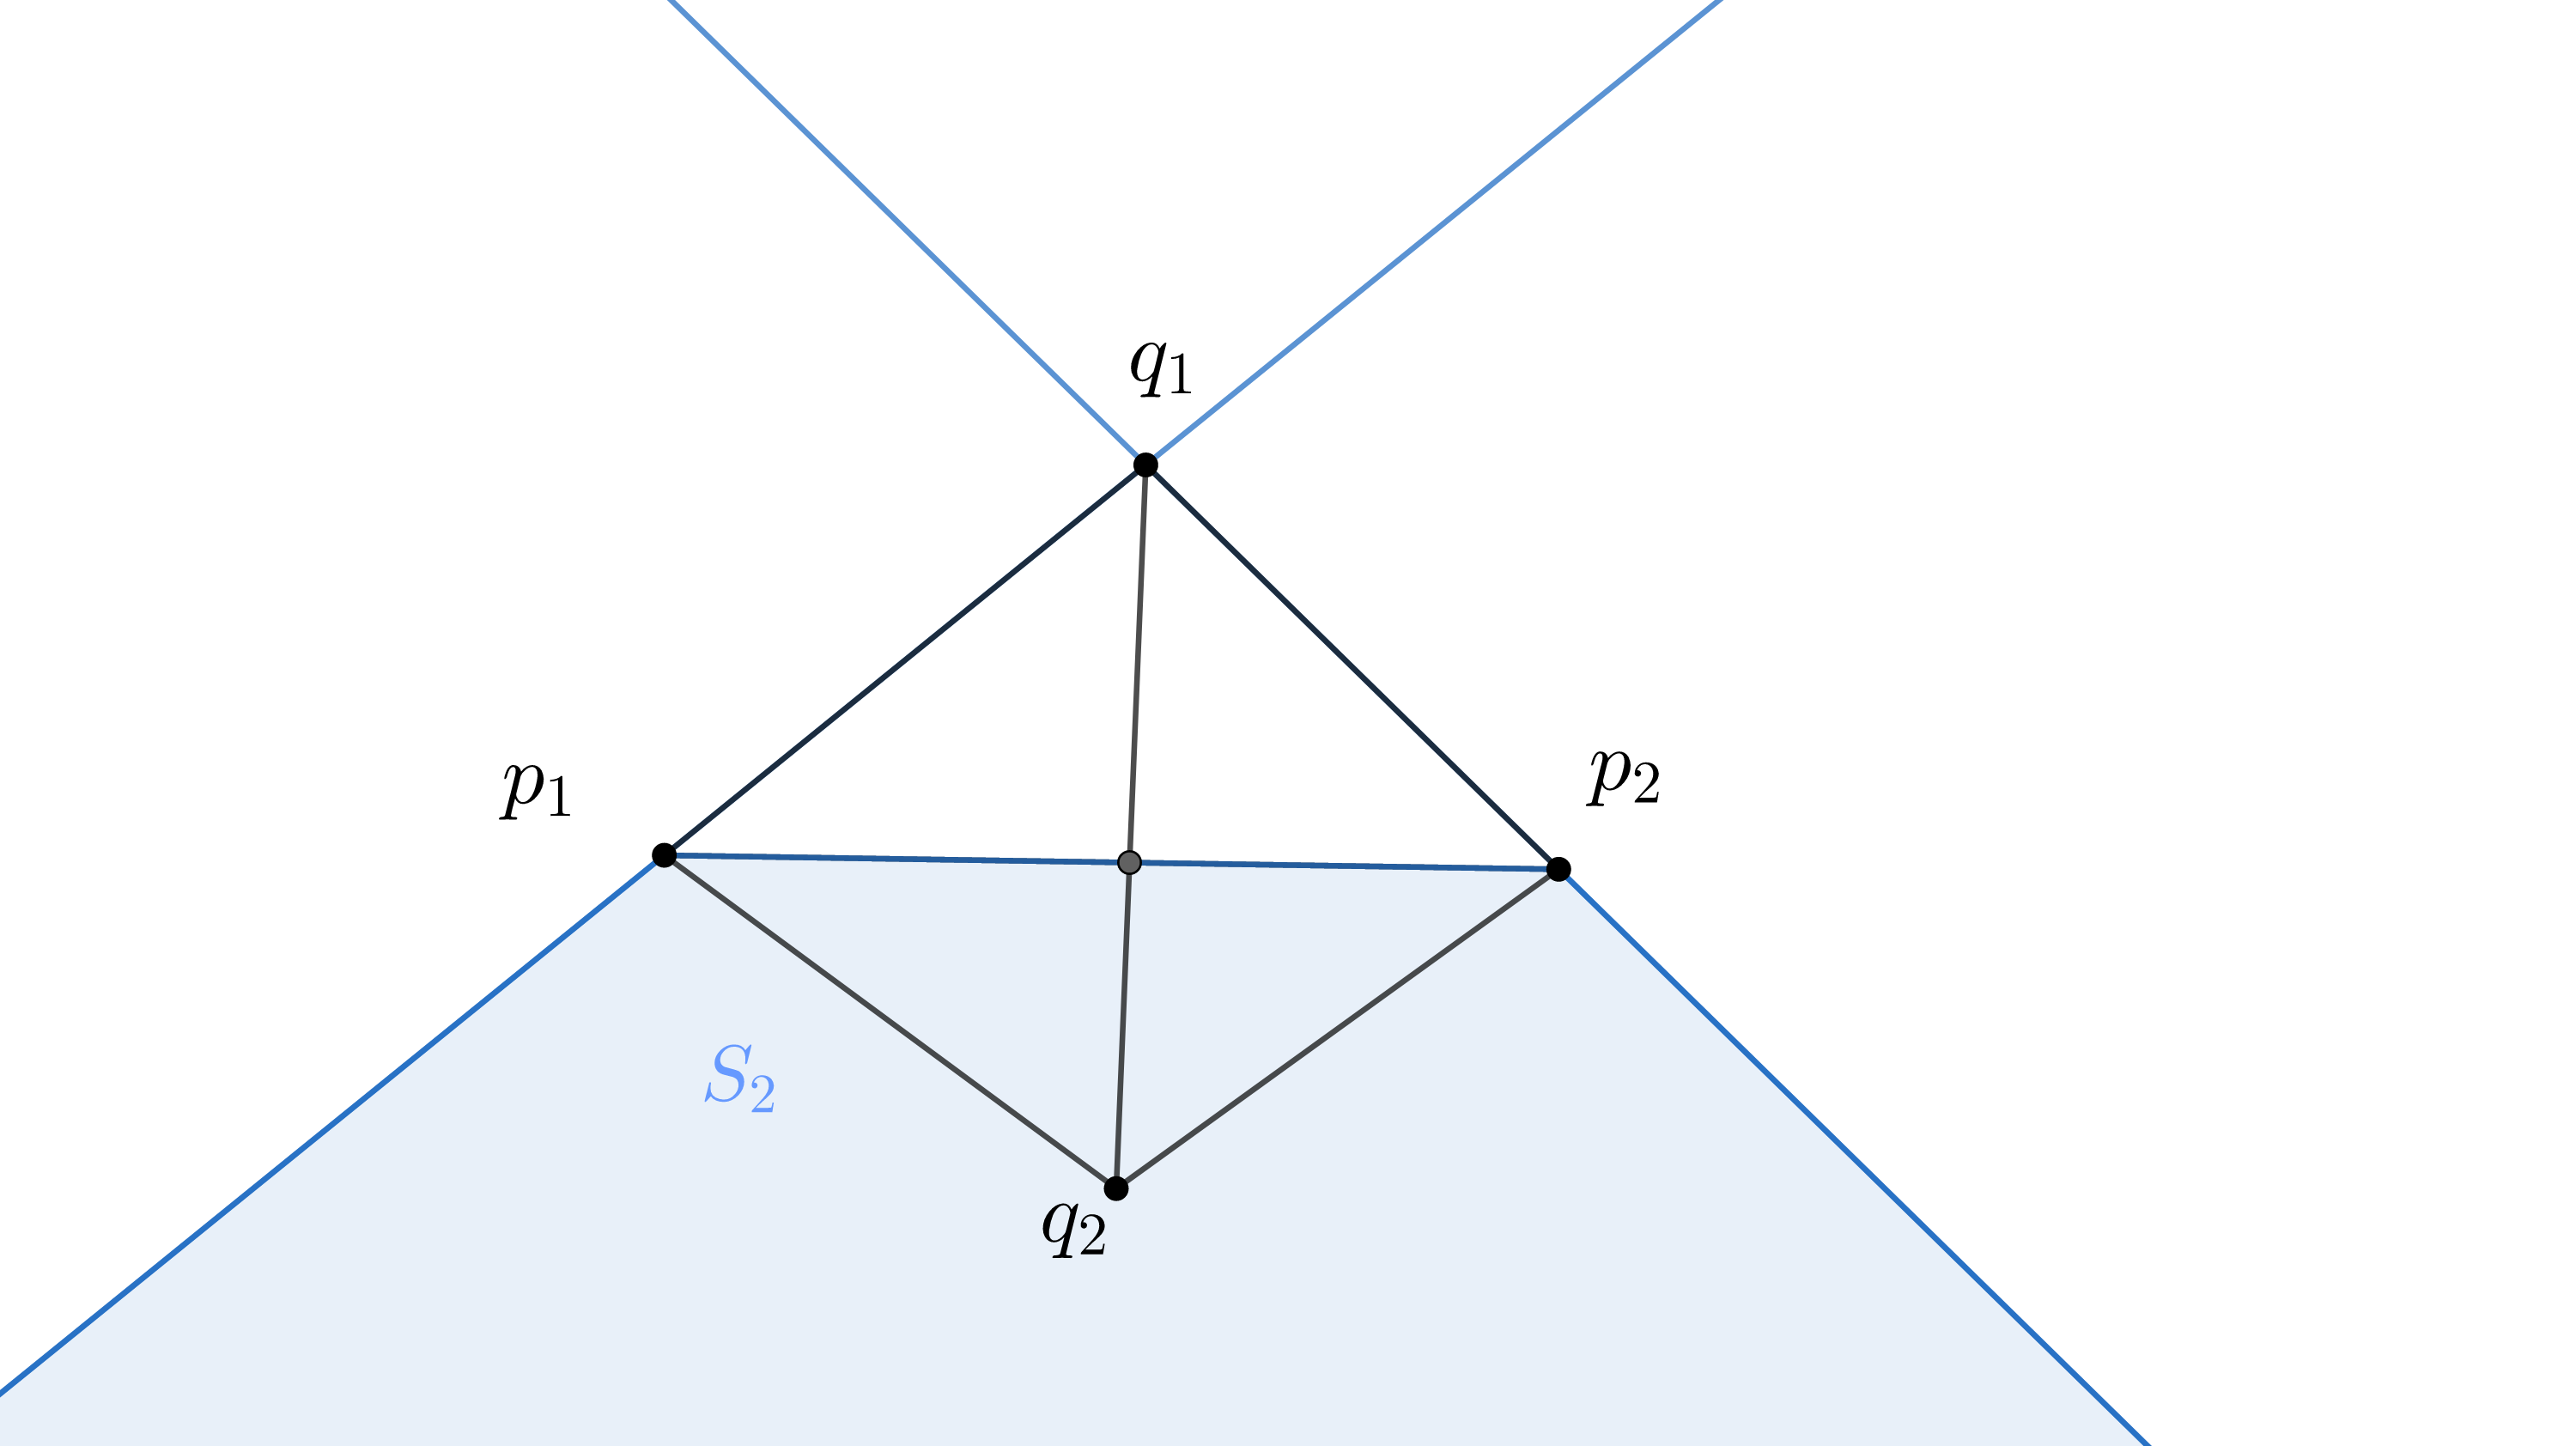
\includegraphics[scale = 0.6]{ge4.png}\\ 
\end{figure} 
Για το δεύτερο σκέλος της άσκησης, καλούμαστε να προσδιορίσουμε αν δύο τμημάτα $\overrightarrow{p_1p_2}$ και $\overrightarrow{p_1p_2}$ τέμνονται. Με βάση το παραπάνω, αρκεί να δείξουμε οτι οτι το πολύγονο $[p_1,q_1,p_2,q_2]$ είναι κυρτό.
\begin{figure}[H]

    \centering
    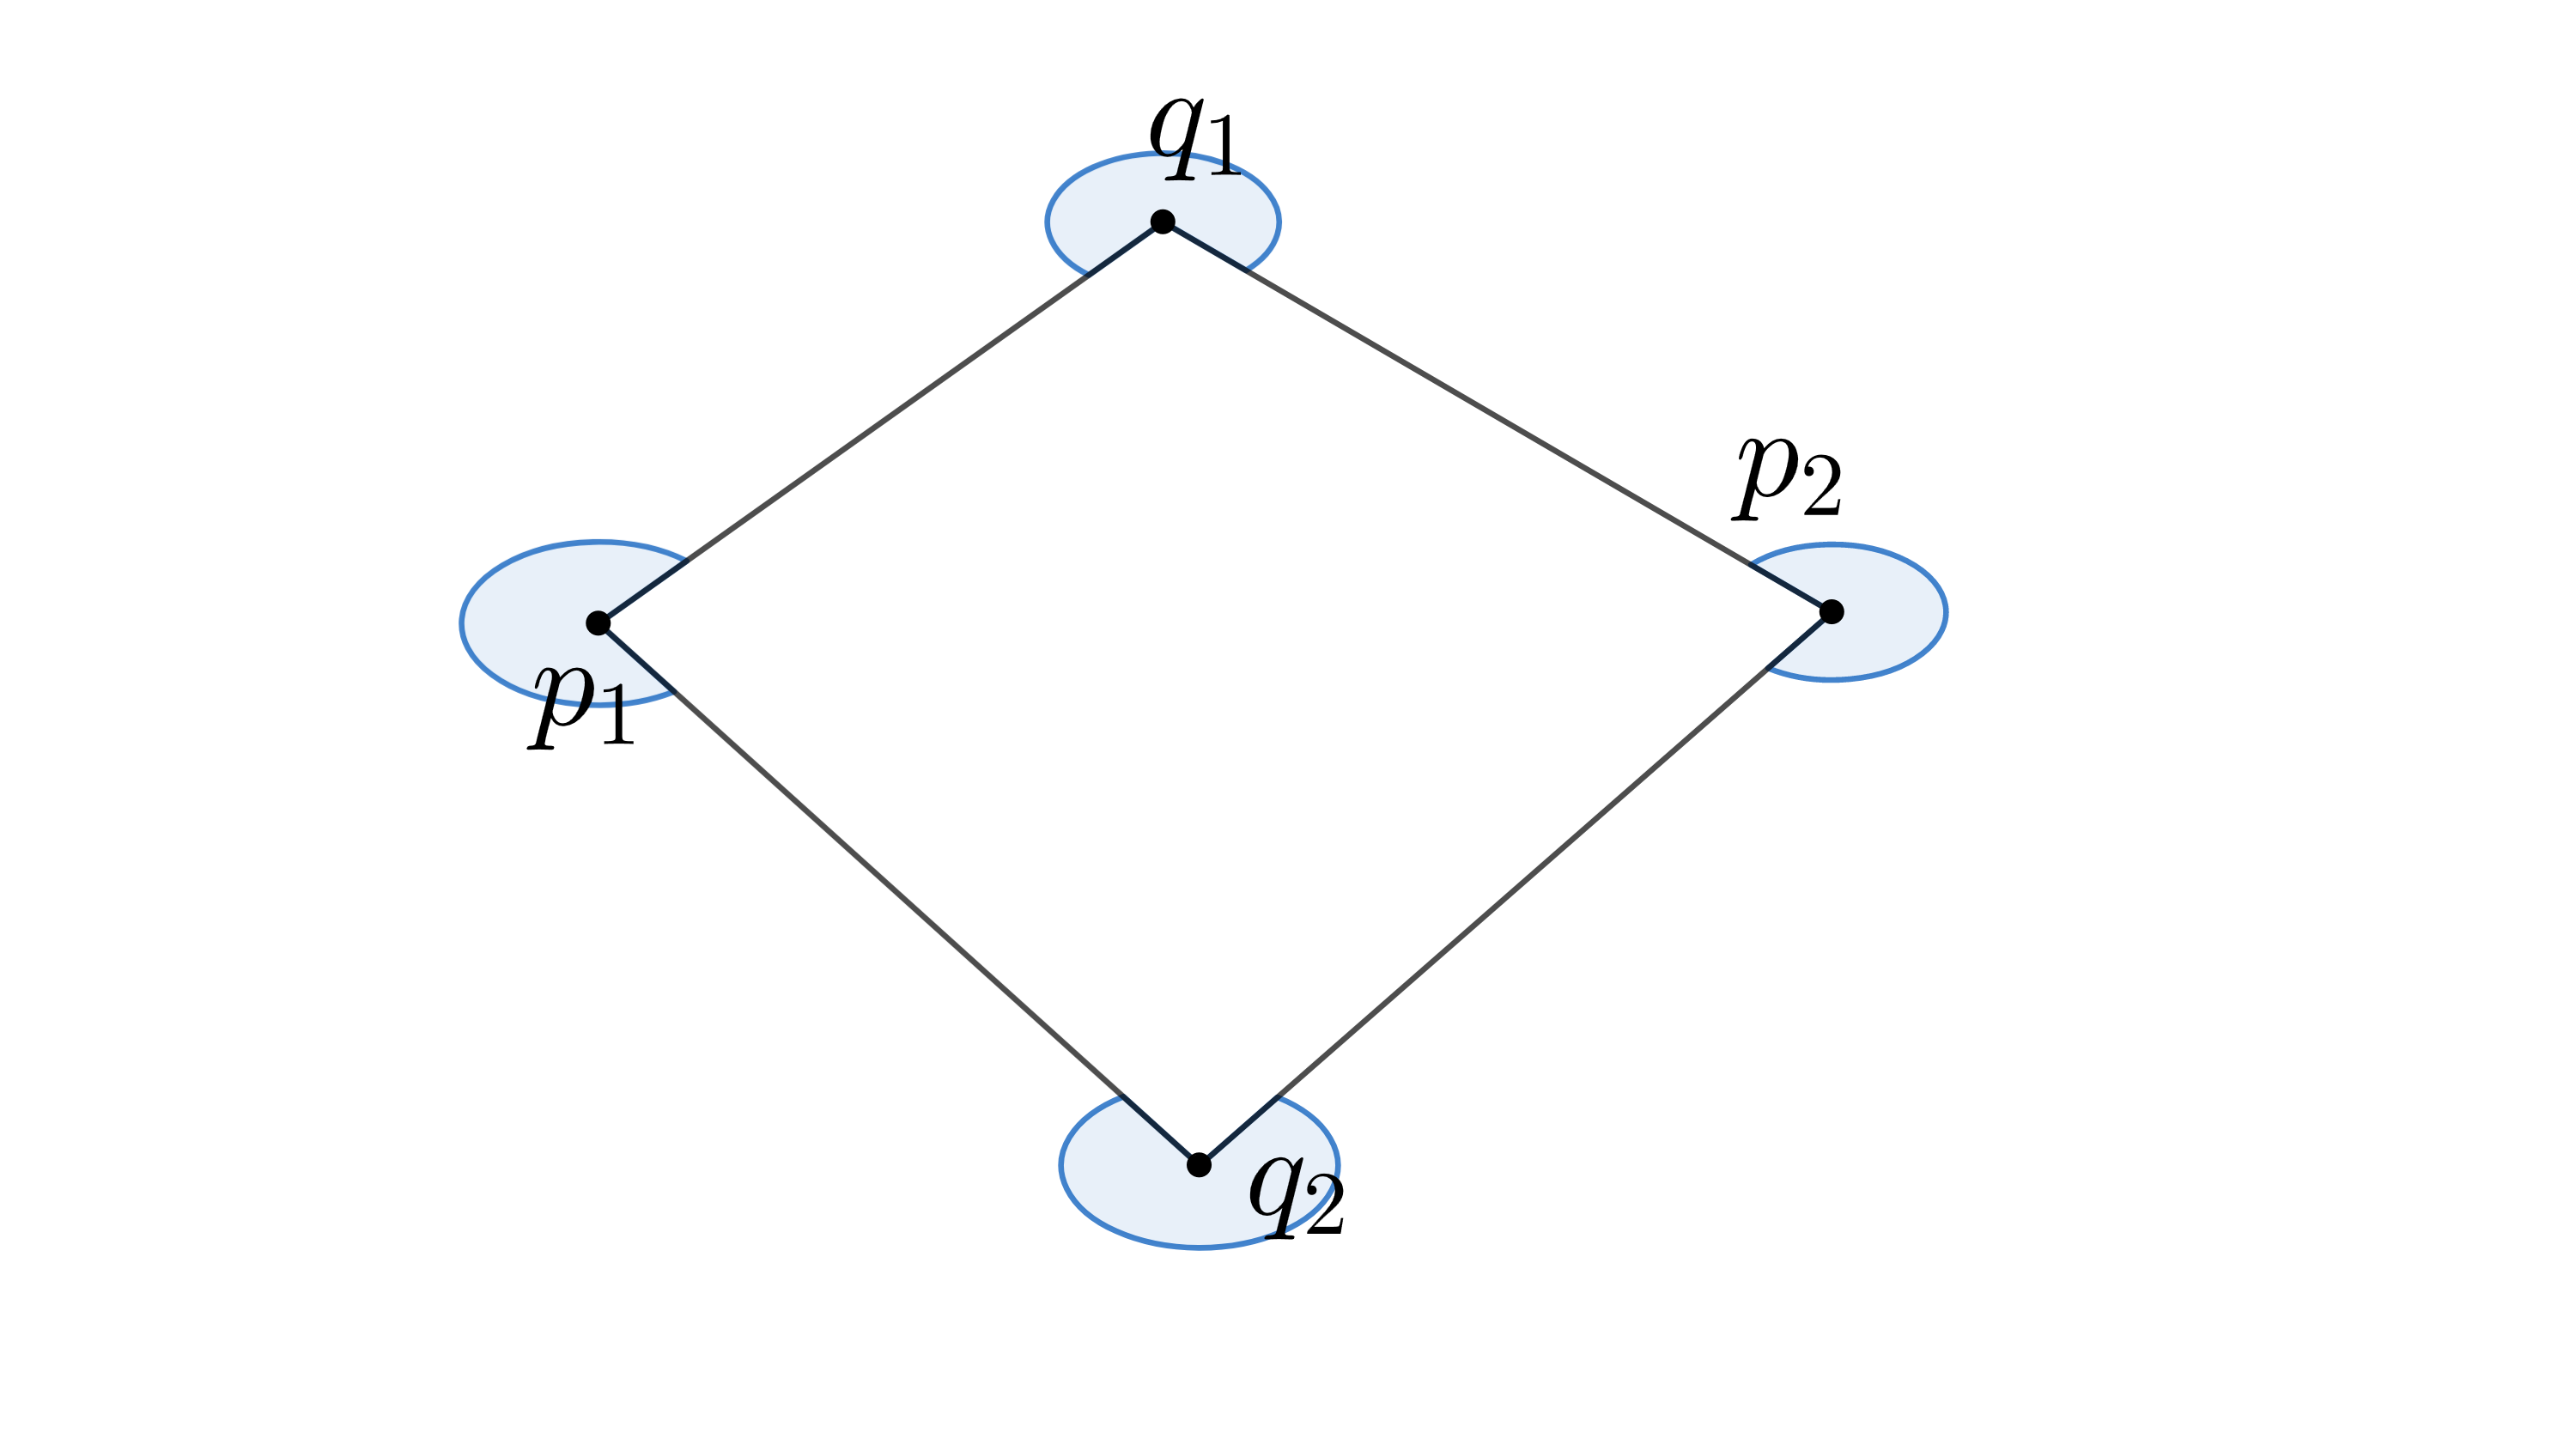
\includegraphics[scale = 0.7]{geogebra-export(2).png}\\ 
\end{figure} 
Ενας τρόπος θα ήταν προσδιορίσουμε
το κύρτο περίβλημα των σημείων $p_1,p_2,q_1,q_2$ με τον αλγίριθμο \textlatin{Jarvis march} και εάν ώς \textlatin{convex hall} προκύψει η ακολουθία $[p_1,q_1,p_2,q_2]$ τότε ξέρουμε οτι το πολύγονο $[p_1,q_1,p_2,q_2]$ είναι κυρτό.\\

Ως Εναλλακτική λύση μπορούμε να ελέγξουμε αν οι τέσσερις γωνίες που σχηματίζονται απο τα τέσσερα σημέια ($\hat{p_1q_1p_2}, q_1\hat{p_2}q_2, p_2\hat{q_1}p_1,q_2\hat{p_1}q_1$) έχουν την ίδια φορά (δεξιόστροφή ή αριστερόστροφη). Aναλυτικά :
\begin{enumerate}
    \item Τοποθετούμε τα σημεία $p_1,q_1,p_2,q_2$  σε μια λίστα \textlatin{list} (με αυτήν την σειρά)
    \item Θέτω $a = list[0],\; b=list[1],\;c=list[2]$  και υπολογίζω το πρόσημο του \textlatin{cross product} $\overrightarrow{ab}\times\overrightarrow{bc}$
    \item Αρχικοποιώ $i=1$ 
    \item Θέτω $a = list[i],\; b=list[i+1],\;c=list[i+2]$  και υπολογίζω το πρόσημο του \textlatin{cross product} $\overrightarrow{ab}\times\overrightarrow{bc}$
    \item Εάν το πρόσημο στο βήμα 4 διαφέρει απο το πρόσημο στο βήμα 2 τότε τερματίζω και επιστρέφω \textlatin{FALSE}. Eάν το πρόσημοστο βήμα 4 είναι ίδιο με το πρόσημο στο βήμα 2 τότε αυξάνω το $i$ ($i=i+1$) και επιστρέφω στη βήμα 4
    \item Συνεχίζω εώς και $i=3$.
\end{enumerate}
Εάν γίνουν τρείς επαναλήψεις χωρίς να τερματίσει στο βήμα 4 (δήλαδή αν ολά τα πρόσημα είναι ίδια), τότε επιστρέφω \textlatin{TRUE}\\
\rule{\textwidth}{.5pt}
\section*{Άσκηση 3}
Σύμφωνα με το \textlatin{hyperplane separation theorem}, αν $S_1,S_2$ δύο κυρτά και διακριτά (μή τεμνόμενα) σύνολα, τότε υπάρχει υπερεπίπεδο ${\bf a}^T{\bf x} = b$ το οποίο να τα διαχωρίζει. Στο πρόβλημα της άσκησης βρίσκει εφαρμογή ώς εξής:\\
Αν ορίσουμε ώς σύνολο $S_1$ το σύνολο τών σημείων $(a_i,c_i)$ και ώς $S_2$  το σύνολο τών σημείων $(a_i,b_i)$, αρκεί να δείξουμε οτι οι κυρτές θήκες των $S_1$ και $S_2$ ($\mathcal{CH}(S_1)\textnormal{ και } \mathcal{CH}(S_2)$) δεν τέμνονται. Τότε σύμφωνα με το 
\textlatin{hyperplane separation theorem}, θα υπάρχει ευθεία που να τις διαχωρίζει και συνεπώς θα υπάρχει ευθεία που να τέμνει όλα τα κάθετα τμήματα $(a_1,b_i,c_i)$

\begin{figure}[H]

    \centering
    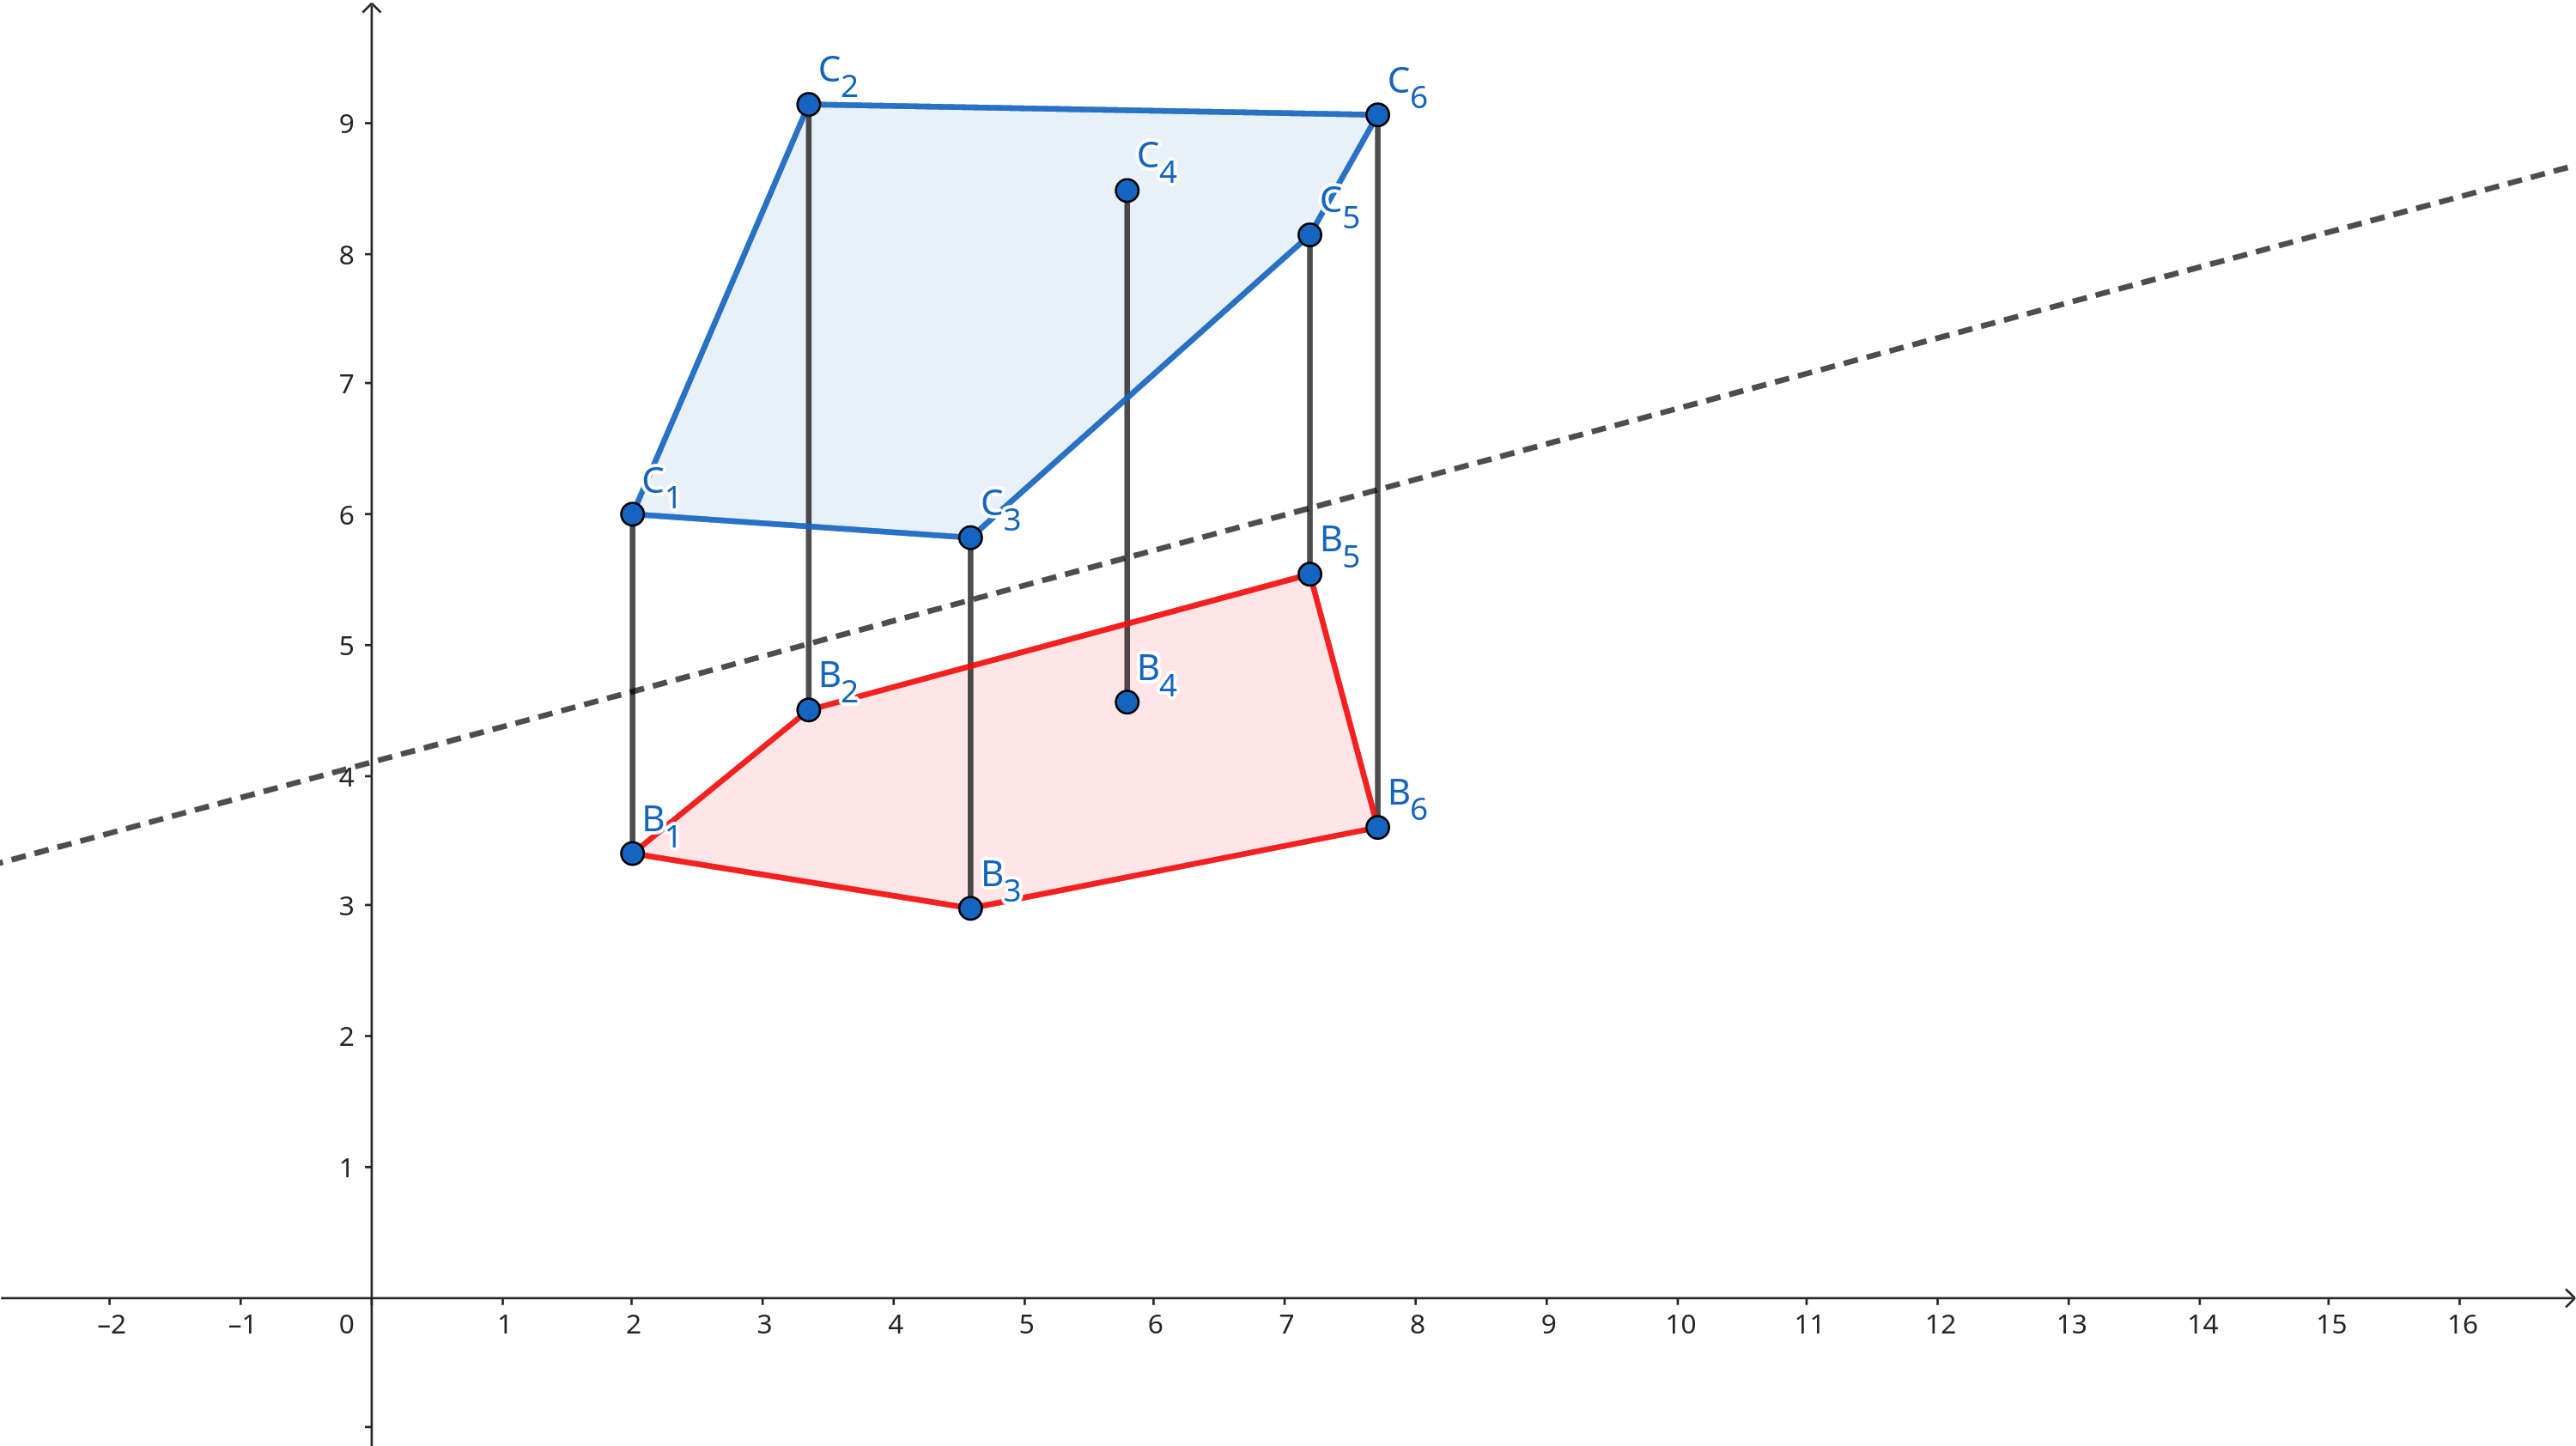
\includegraphics[scale = 0.85]{GE6.png}\\ 
\end{figure} 
Ένας $O(n\log n)$ ο οποίος λύνει το πρόβλημα εκμεταλευόμενος τον παραπάνω ισχυρισμό είναι ο εξής:
\begin{enumerate}
    \item  Αρχικά βρίσκουμε τα κυρτά περιβλήματα των $S_1$ και $S_2$ χρησιμοποιώντας τον αλγόριθμο \textlatin{Jarvis march} σε χρόνο $O(n\log n)$ 
    \item Έπειτα θέλουμε να προσδιορίσουμε αν τα $\mathcal{CH}(S_1)$ και $\mathcal{CH}(S_2)$ είναι διακριτά σε χρόνο $O(n\log n)$. Ένα τρόπος να το κάνουμε είναι να χρησιμοποιήσουμε τον αλγόριθμο 
            \textlatin{T. Chan} ο οποίος βρίσκει τις τομές μεταξύ \textlatin{red/blue} τμημάτων. Ορίζοντάς ώς σύνολο \textlatin{blue} τμημάτων $B$ το $\mathcal{CH}(S_1)$ και ώς σύνολο \textlatin{red} τμημάτων $R$ το $\mathcal{CH}(S_2)$ (όπως φαίνεται στο σχήμα παραπάνω),
            ο αλγόριθμος θα βρεί τις τομές τους σε χρόνο $O(n\log n +k)$ όπου $n$ το πλήθος τών τμήματων και $k$ το πλήθος τών τομών. Αλλά λόγω της τοπολογίας τών τμημάτων, ο αριθμός τών τομών δεν θα μπορεί να υπερβαίνει το $n$ άρα η πράγματική πολυπλοκότητα θα είναι $Ο(n\log n + n) = O(n\log n)$. Ο 
            αλγόριθμος απαιτεί τα τμήματα στο εσωτερικό του κάθε συνόλου να μήν τέμνοντα αλλα επιτρέπει να εφάπτονται στα άκρα τους, οπότε μπόρει να εφαρμοστεί στα δικά μας σύνολα $R$  και $B$
    \item Αν ο αλγόριθμος \textlatin{T. Chan} δεν βρεί καμία τομή τότε επιστρέφουμε \textlatin{TRUE} καθώς τα σύνολα $\mathcal{CH}(S_1)$ και $\mathcal{CH}(S_2)$ θα είναι διακριτά. Διαφορετικά επιστρέφουμε \textlatin{FALSE}
        \end{enumerate}
    Η τελική πολυπλοκότητα του αλγορίθμου θα είναι 
    $$ \textnormal{\textlatin{Jarvis march}} + \textnormal{\textlatin{T. Chan}} = O(n\log n) + O(n \log n) = O(n\log n)$$
\rule{\textwidth}{.5pt}
\section*{Άσκηση 4}
Έστω σύνολο πεπερασμένων σήμειων με κυρτό περίβλημα με περίμετρο $P_1$. Έστω οτι υπάρχει περιμετρικό πολύγονο με περιμέτρο $P_2<P_1$ το οποίο περνάει αποο σημείο $C$ που παραβιάζει την κυρτότητα του περιβλήματος με περίμετρο $P_2$, όπως φαίνεται στο παρακάτω σχήμα.
\begin{figure}[H]

    \centering
    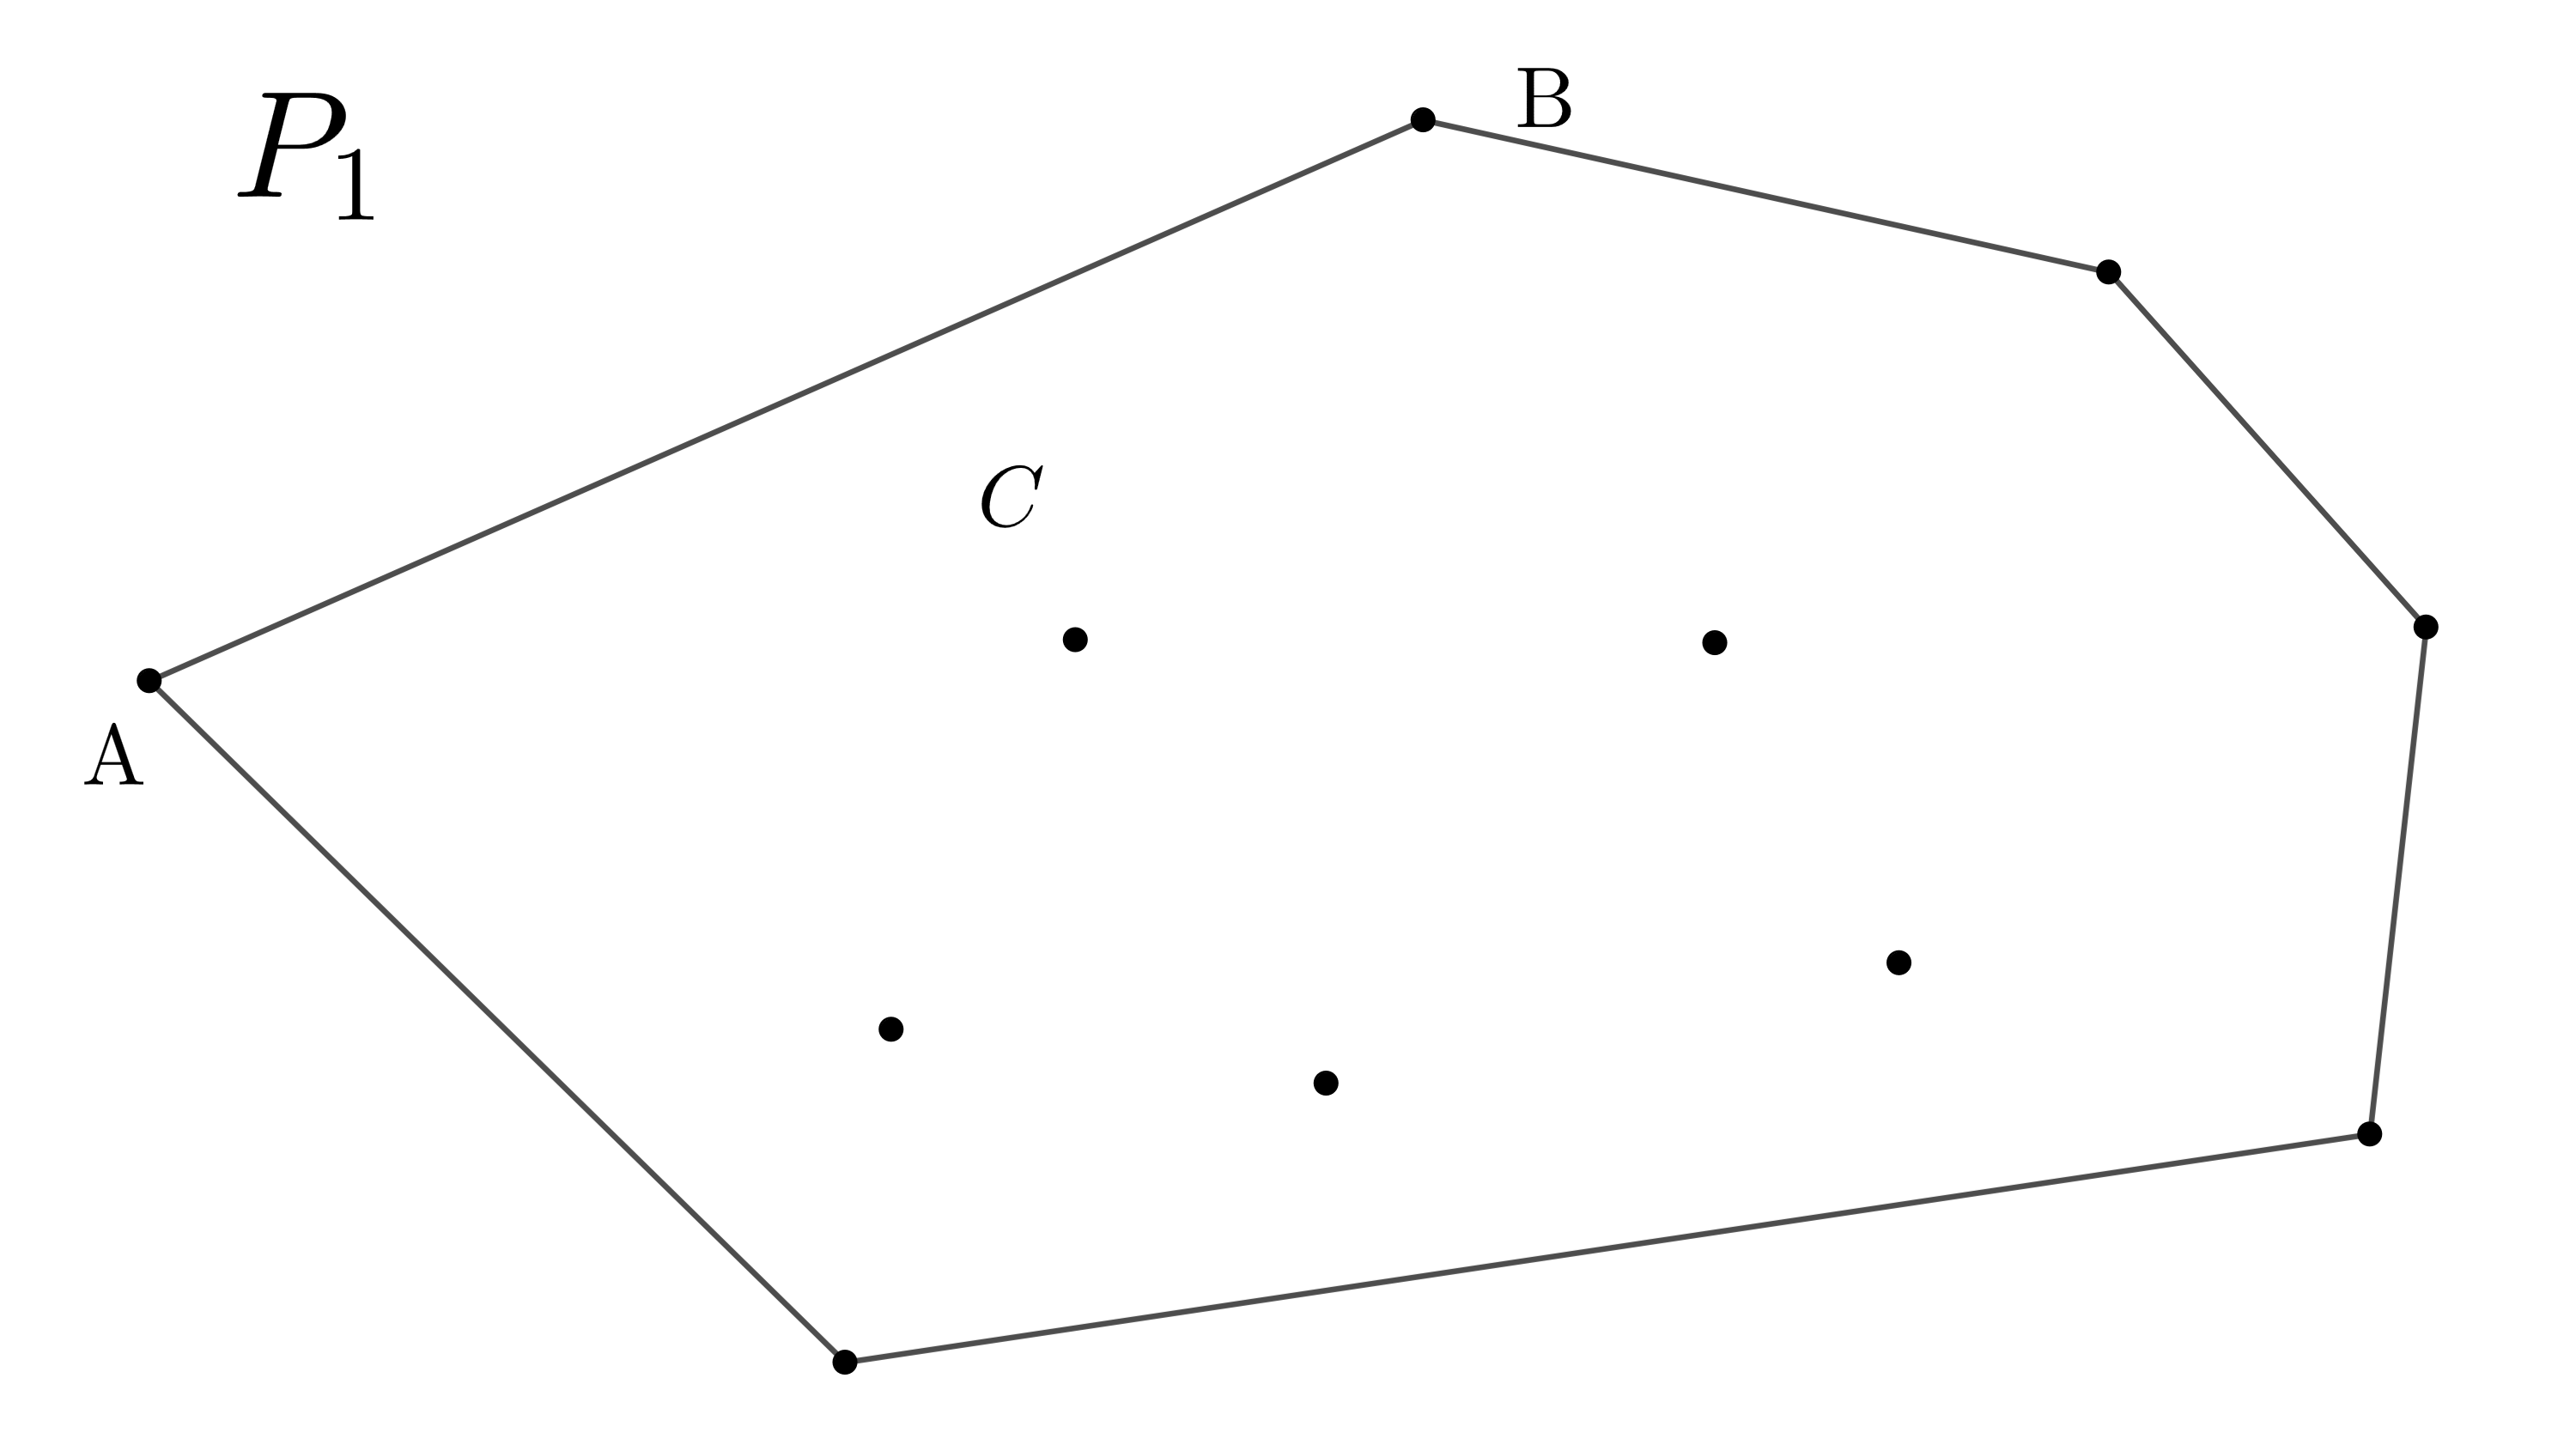
\includegraphics[scale = 1.1]{ge8.png}
    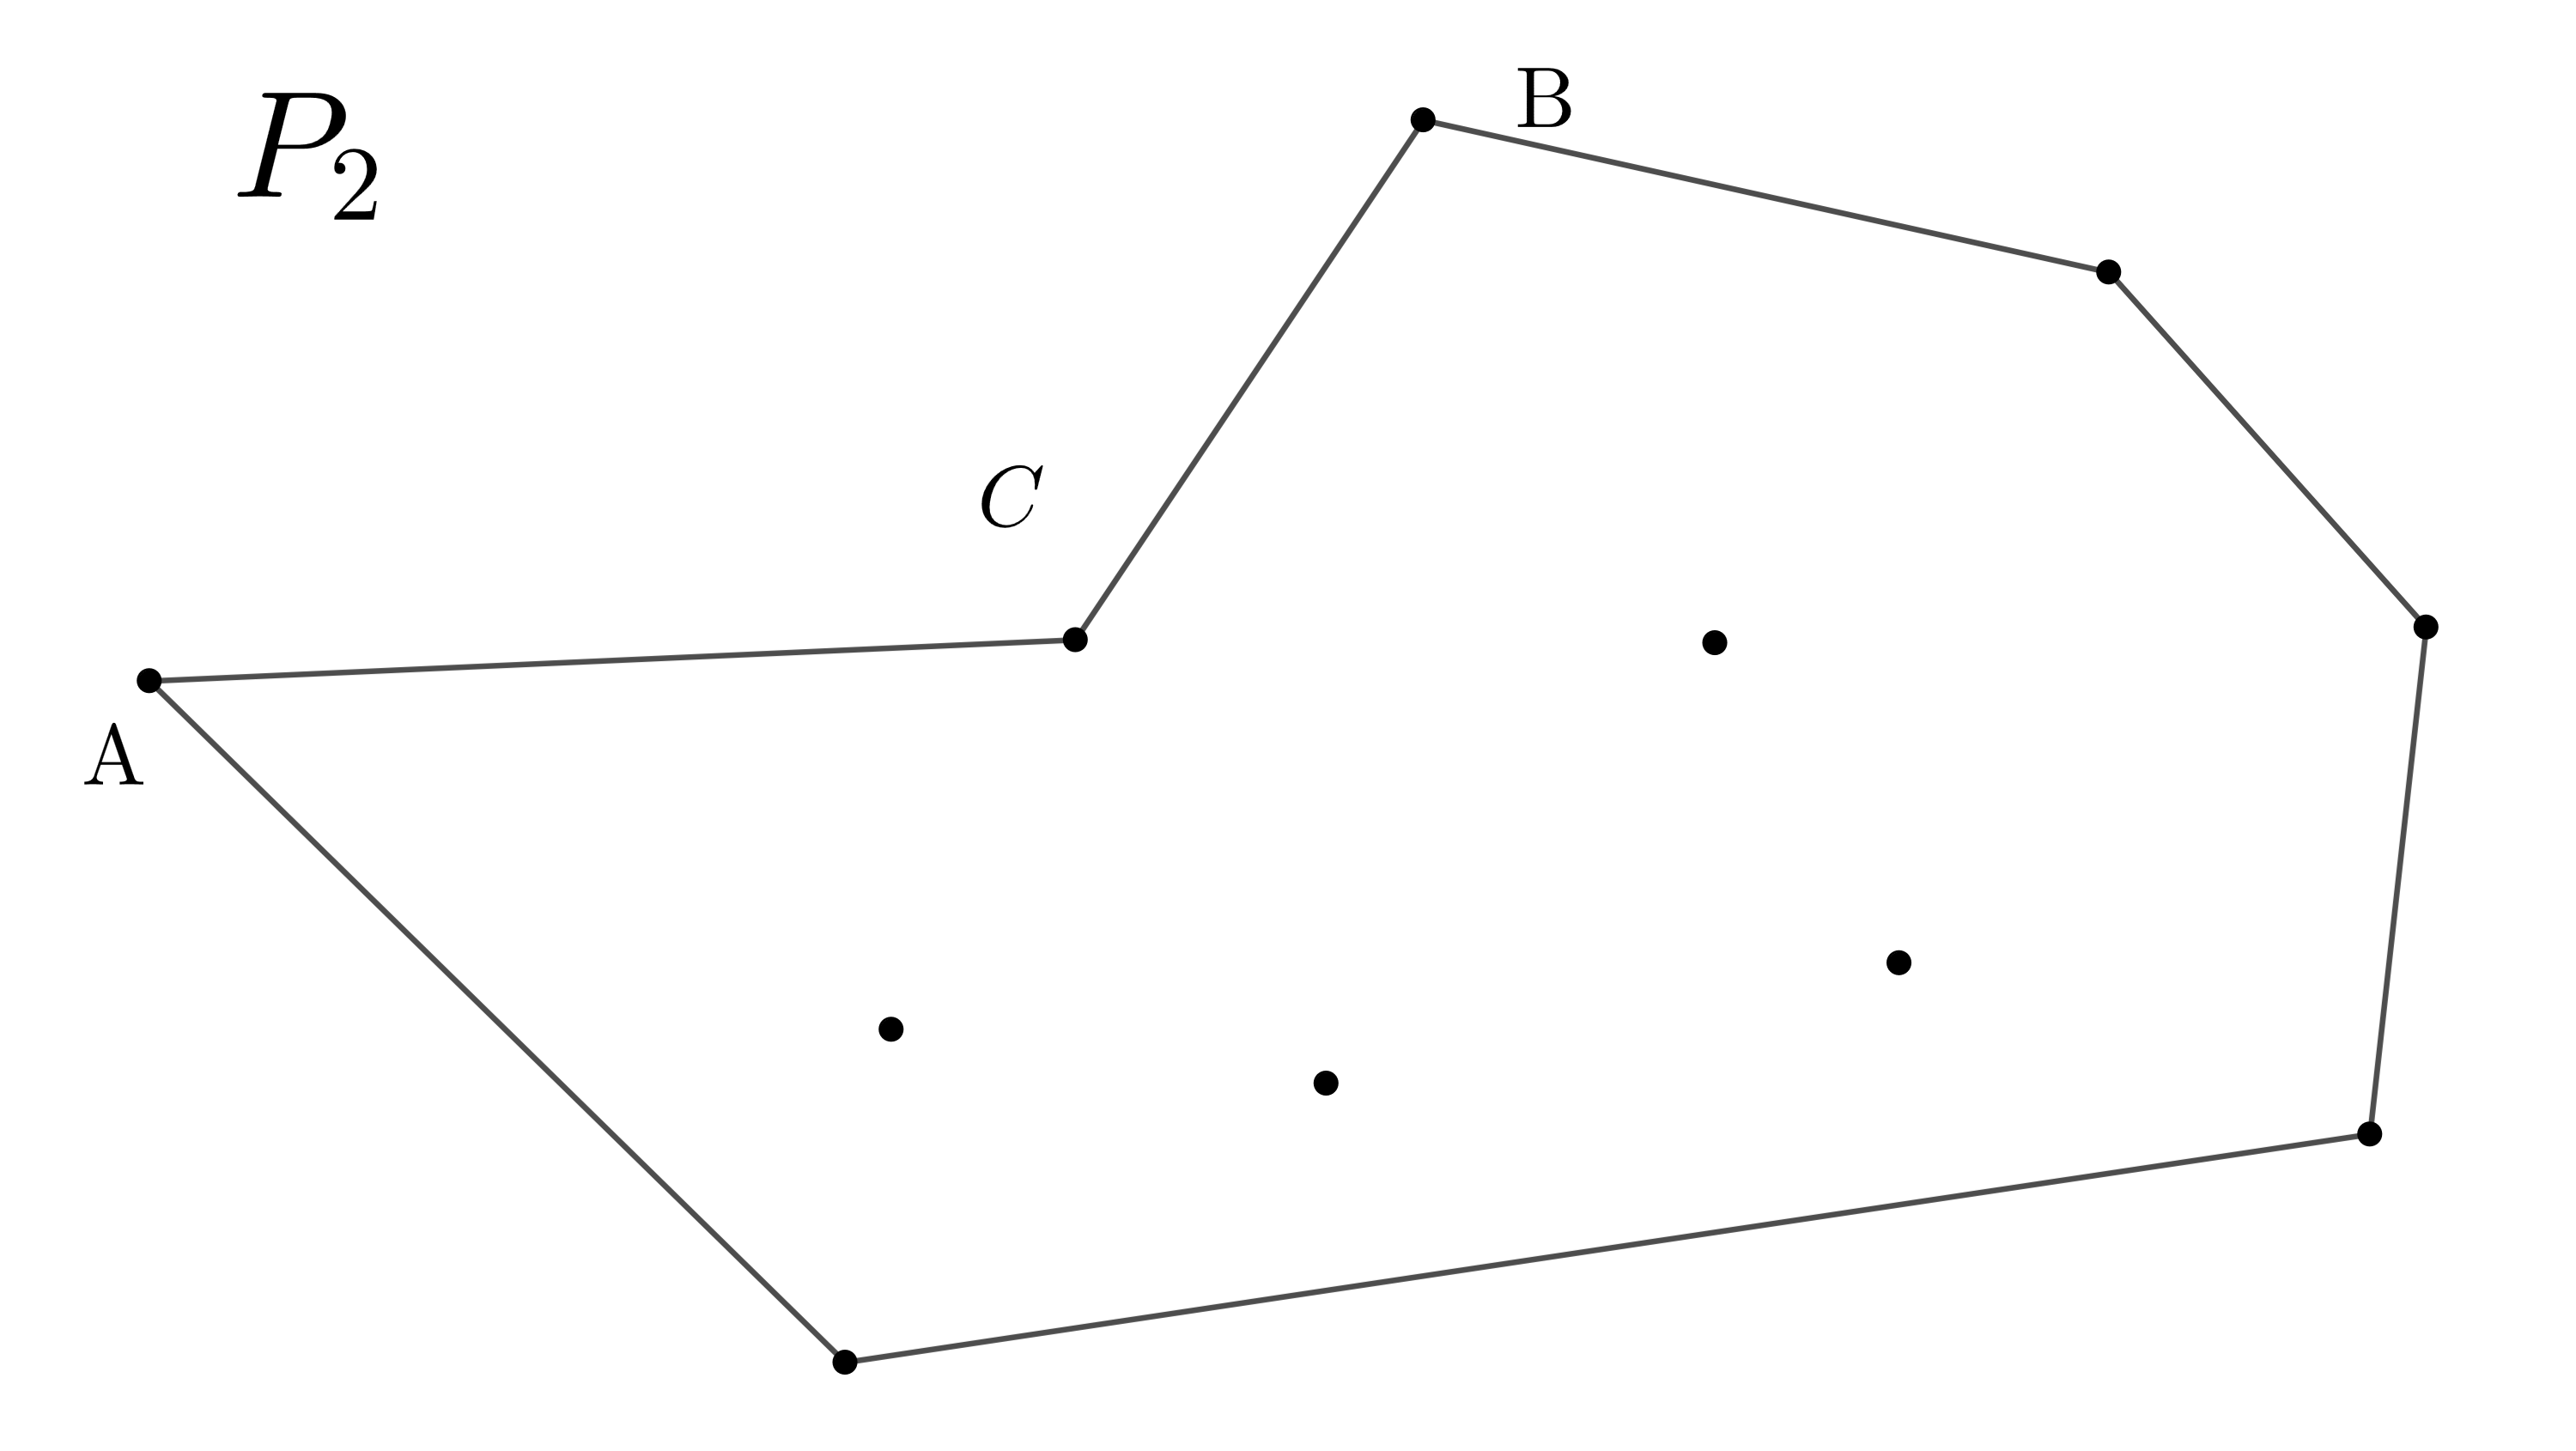
\includegraphics[scale =1.1]{ge7.png}
\end{figure} 
Παρατηρούμε οτι $P_2 = P_1 - \|AB\| + \|AC\| + \|CB\|$ Άρα 
$$ P_2<P_1 \Leftrightarrow P_1 - \|AB\| + \|AC\| + \|CB\| <P_1\Leftrightarrow \|AC\| + \|CB\|< \|AB\|$$
Το τελικό συμπέρασμα είναι άτοπο καθώς παραβιάζειτην τριγωνική ανισότητα. Αρα δεν μπορεί να υπάρξει το πολύγονο με περίμετρο $P_2$ συνεπώς το κυρτό περίβλημα είναι το περίβλημα με την ελάχιστη περίμετρο.\\
\rule{\textwidth}{.5pt}
\section*{Άσκηση 5}
To επίπεδο $P$ που ορίζεται απο τα σημεία $\bf p_1,p_2,p_3 \in \mathbb{R}^3$ περιγράφεται ως:
$$P:\;\;\;{\bf p_1}+\lambda_1({\bf p_2 - p_1})+\lambda_2({\bf p_3 - p_2}) \;\;\; \textnormal{για }\;\; \lambda_1,\lambda_2 \in \mathbb{R}$$
Θέλουμε να βρούμε το σημείο τομής του $P$ με την ημιευθεία $\boldsymbol{\alpha} + \lambda {\bf D}\;\; \lambda>0$ λύνοντας την εξίσωση 
$$ \boldsymbol{\alpha} + \lambda {\bf D} = {\bf p_1}+\lambda_1({\bf p_2 - p_1})+\lambda_2({\bf p_3 - p_2}) \Leftrightarrow   \lambda {\bf D} -\lambda_1({\bf p_2 - p_1})-\lambda_2({\bf p_3 - p_2})= {\bf p_1} -\boldsymbol{\alpha} \Leftrightarrow$$
$$ \begin{bmatrix}{\bf D}&&{\bf p_1 - p_2}&&{\bf p_2 - p_3}\end{bmatrix} \begin{bmatrix*}
    \lambda\\
    \lambda_1\\
    \lambda_2
\end{bmatrix*} = {\bf p_1} -\boldsymbol{\alpha}$$

Για να υπάρχει σημείο τομης της ημιευθείας και του επιπέδου θα πρέπει το παραπάνω σύστημα γραμμικών εξισώσεων να έχει λύση ως προς $\boldsymbol{\lambda} = (\lambda, \lambda_1,\lambda_2)$  και να προκύψει $\lambda>0$ . Απο εκεί και πέρα προκειμένου το σημείο τομής να 
βρίσκεται στο εσωτερικό του τριγώνου $\bf p_1p_2p_3$ θα πρέπει στην λύση του συστήματος να προκύψουν $0<\lambda_1<1$ και $0<\lambda_2<\lambda_1$.\\
\begin{figure}[H]

    \centering
    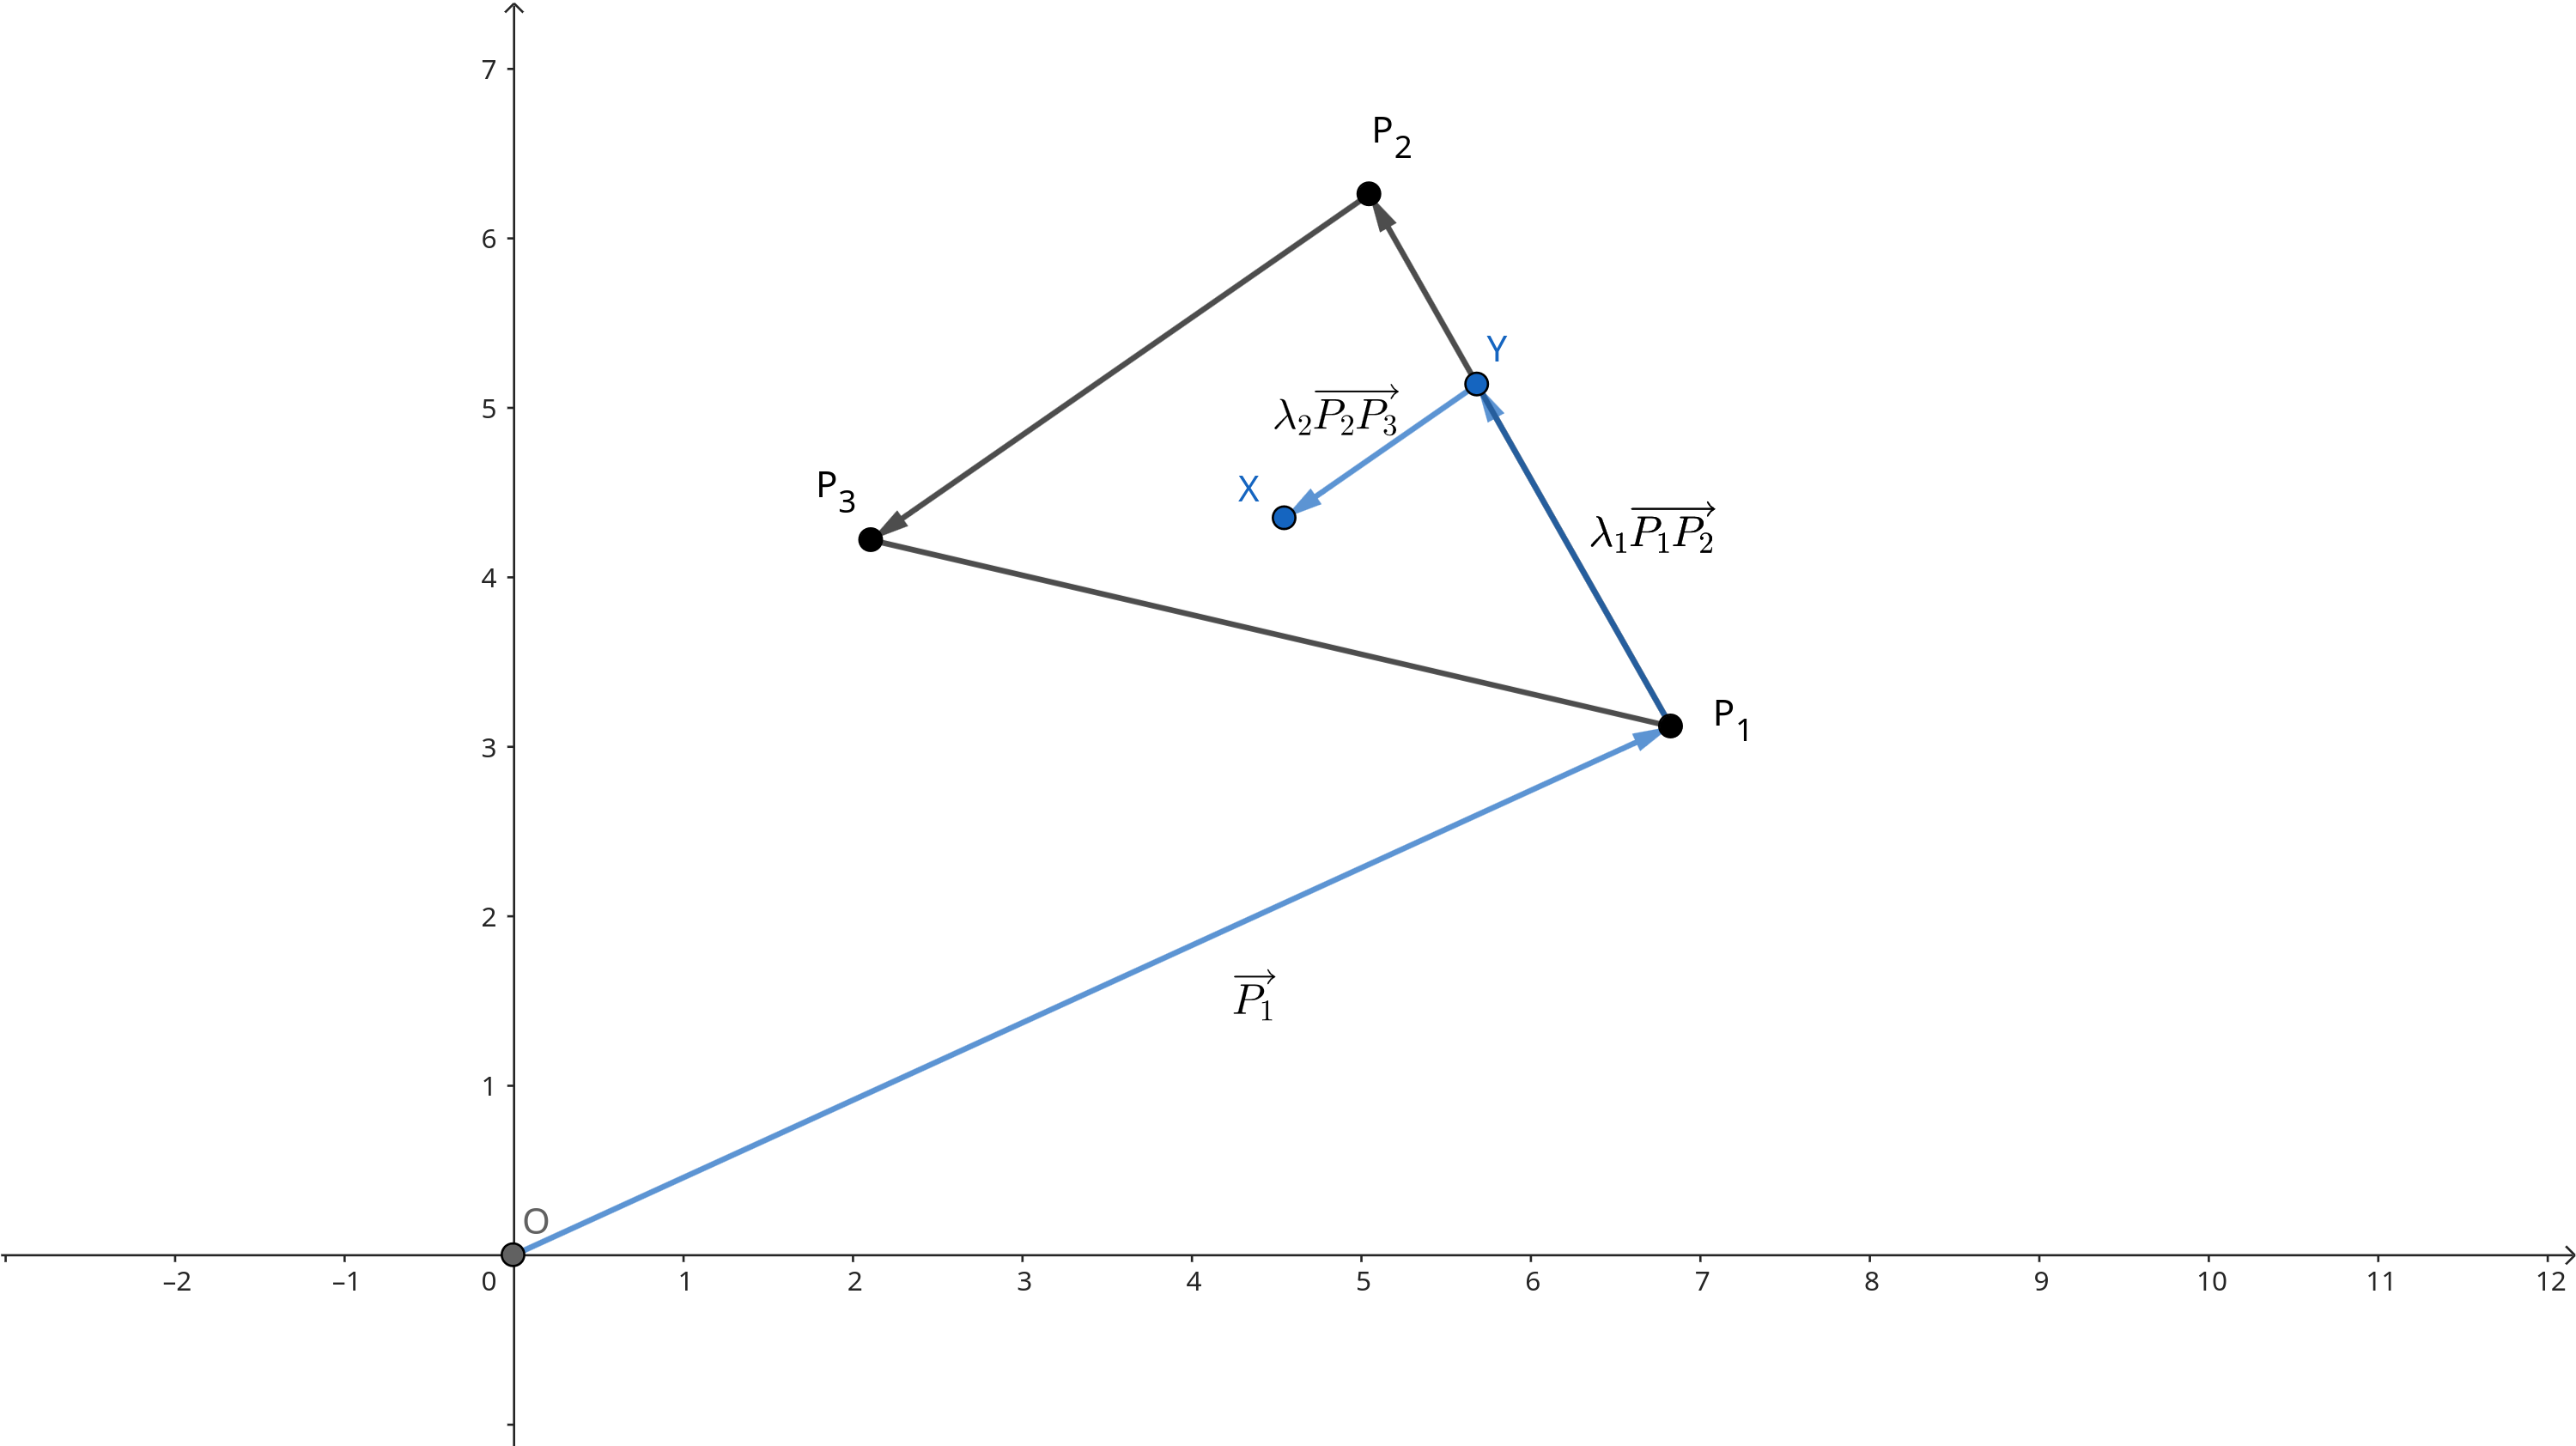
\includegraphics[scale = 1]{γε9.png}
\end{figure} 
Όπως φαίνεται στο παραπάνω σχήμα εάν $\bf X$ το σημείο τομής και  $\lambda_1 = \lambda_2$ τότε το τρίγωνο $\bf P_1YX$ είναι όμοιο με το $\bf P_1P_2P_3$, όποτε το σημείο τομής $\bf X$ πέφτει πάνω στο τμήμα $\overline{P_3P_1}$. Εάν $\lambda_1 < \lambda_2$ τότε το $\bf X$ πέφτει εκτός του τριγώνου. Άρα πρέπει $\lambda_1 > \lambda_2$.\\
Εφόσον λυθεί το σύστημα, το σήμειο τομής θα προσδιρίζεται απο την σχέση 
$${\bf x} = {\bf p_1}+\lambda_1({\bf p_2 - p_1})+\lambda_2({\bf p_3 - p_2}) \;\;\;\textnormal{για}\;\; \lambda_1\in (0,1) \;\;\textnormal{και}\;\;\lambda_2\in (0,\lambda_1)$$
\rule{\textwidth}{.5pt}
\end{document}